\graphicspath{{main/chapter2/fig/}}

\chapter{Algorithms and Efficient Methods of Receiver}

\section{Strategy for Optimizations}

\subsection{Algorithmic Simplifications}

\subsection{Memory Data Layer}

\subsection{Quantification}

\subsection{Vectorization~\cite{Cassagne2018}}

\begin{itemize}
  \item \xmark~le temps d'exécution d'une tâche peut varier entre quelques
    microsecondes et quelques milliseconde -> faible latence -> adapté à la
    vectorisation
  \item \xmark~expliquer les approches intra-trame et inter-trame pour faire du
    SIMD
  \item \cmark~\textbf{état de l'art wrapper SIMD}
  \item \cmark~portabilité (ARM to Xeon Phi)
\end{itemize}

Recent articles have proposed several optimized software decoders, corresponding
to different channel codes : LDPC codes~\cite{LeGal2015,LeGal2016}, polar
codes~\cite{Giard2016b,Sarkis2016,Cassagne2015c,Cassagne2016b}, turbo
codes~\cite{Zhang2012,Wu2013,Cassagne2016a}. All of these works show the
possibility to reach a good level of \textit{performance} by  making extensive
use of SIMD (Single Instruction Multiple Data) units. This is often achieved at
the price of a reduced \textit{flexibility}, by resorting to specific
intrinsics, or by making assumptions on the data types. However, these decoders
should be implemented in a single source code, in which the following parameters
could be changed at runtime: the channel code type, the decoding algorithm, the
number of decoding iterations, the data format, etc. Another important aspect is
the \textit{portability} of the source code on different hardwares (Intel x86,
Xeon KNL and ARM) and the possibility to use different instruction sets
(\verb|SSE|, \verb|AVX|, \verb|AVX-512|, \verb|NEON|). These three constraints
(performance, flexibility, portability) push towards the use of a SIMD library
that helps in the abstraction of the SIMD instruction sets, while still allowing
a fine grain tuning of performance.

We propose in this thesis a new \Cxx SIMD wrapper, covering the needs in terms
of expressiveness and of performance for the channel codes. Our contributions
are:
\begin{itemize}
  \item A portable and high performance  \Cxx SIMD wrapper called \MIPP, for
    \verb|SSE|, \verb|AVX|, \verb|AVX-512| and \verb|NEON| instruction sets;
  \item An implementation of several channel codes with this wrapper. We
    present the main advantages of \MIPP in this context;
  \item A comparison with other state-of-the-art SIMD wrappers on a Mandelbrot
    code, demonstrating that the code based on \MIPP has similar performance as
    hand-written intrinsics.
\end{itemize}
\MIPP programming model is not too far from intrinsics, allowing a good control
on performance, but still provides an abstraction on the basic types used in
vectors (ranging from double to byte) and complex operations (parametric
reductions, log, exponential, ...).

The \longMIPP library (\MIPP) is a portable wrapper for SIMD intrinsics written
in the \Cxx language. It relies on \Cxx compile-time template specialization
techniques to replace supported generic functions with inline calls to their
intrinsics counterpart, for a given instruction set. While \MIPP is mostly
written in \Cxy{98}, it still requires \Cxy{11}-compliant compiler due to the
use of convenient features such as the \verb|auto| and \verb|using| keywords.
\MIPP is Open-source (under the MIT license) and the full code is available on
GitHub\footnote{\MIPP source code: \url{https://github.com/aff3ct/MIPP}}.

\MIPP provides two application programming interface levels. The
\emph{Low Level Interface} (low) implements a basic, thin abstraction layer on
top of the intrinsics. The \emph{Medium Level Interface} (med.), built on top of
\MIPP low, abstracts away more details to lessen the effort from the application
programmer by relying on object encapsulation and operator overloading.

\subsubsection{Low Level Interface}

\MIPP low is built around a unified \verb|mipp::reg| type that abstracts vector
registers. The vector register type represents hardware registers independently
of the data type of the vector elements. \MIPP uses the longest native vector
length available on the architecture. This design choice preserves programmer
flexibility, for instance in situations such as mixing fixed-point and
floating-point operations. \MIPP also defines a \emph{mask} register type
\verb|mipp::msk|, which either directly maps to real hardware masks on
instruction sets that support it (such as AVX-512), or to simple vector
registers otherwise.

\MIPP low then defines a set of functions working with \verb|mipp::reg| and
\verb|mipp::msk|, organized into eight families: memory accesses, shuffles,
bitwise boolean arithmetic, integer operations, float. operations, mathematical
functions, reductions, and mask operations.

In the AVX-512 instruction set, one \textit{regular} vector operation plus one
masking operation can be performed in one CPU clock cycle. For instance, the
following instruction performs \verb|"m ? a+b : src"|, an addition and a masking
operation:
\mint{C++}|__m512 _mm512_mask_add_ps(__m512 src, __mmask16 m, __m512 a, __m512 b);|

\MIPP natively supports such operations with the \verb|mipp::mask| function. The
previous example becomes in \MIPP:
\mint{C++}|mipp::mask<float,mipp::add<float>>(m, src, a, b);|
For instruction sets without masking support, the \verb|mipp::mask| call is
expanded as an operation and a \verb|blend| instead.

\subsubsection{Medium Level Interface}

\begin{listing}
  \inputminted[frame=lines,linenos]{C++}{main/chapter2/src/vectorization/mipp_mli.cpp}
  \caption{Medium Level Interface encapsulation.}
  \label{lst:vectorization_mli}
\end{listing}

The \MIPP Medium Level Interface (\MIPP med.) provides additional expressiveness
to the programmer. \verb|mipp::reg| and \verb|mipp::msk| basic types are
encapsulated in \verb|mipp::Reg<T>| and \verb|mipp::Msk<N>| objects,
respectively. The \verb|T| and \verb|N| template parameters correspond to the
type and the number of elements inside the vector register and the mask
register, respectively. One can notice that in these register objects are typed,
unlike the \MIPP low register basic type. It avoids to write the type when a
\MIPP function is called. The function type can then be directly selected from
the parameter type. Listing~\ref{lst:vectorization_mli} illustrates the
template-based encapsulation, which enables \MIPP to override common arithmetic
and comparison operators.

\MIPP med. also simplifies register loading and initialization operations. The
constructor of the \verb|mipp::Reg| object will call the \verb|mipp::load|
function automatically. Thus, a load in \MIPP low:
\mint{C++}|mipp::reg a = mipp::load<float>(aligned_ptr);|
can be simplified into:
\mint{C++}|mipp::Reg<float> a = aligned_ptr;|
with \MIPP med. level. An initializer list
can be used with a \MIPP med. vector register:
\mint{C++}|mipp::Reg<float> a = {1.f, 2.f, 3.f, 4.f};|
Likewise, a scalar assigned to a vector sets all elements to
this value.

\subsubsection{Implementation Details}
\label{subsec:implem}

\MIPP targets \verb|SSE2|, \verb|SSE3|, \verb|SSSE3|, \verb|SSE4.1|,
\verb|SSE4.2|, \verb|AVX|, \verb|AVX2|, \verb|FMA3|, \verb|KNCI|,
\verb|AVX-512F| and \verb|AVX-512BW| instruction sets on x86 and related
architectures, as well as \verb|NEON|, \verb|NEONv2|, \verb|NEON64| and
\verb|NEON64v2| on ARM. It can easily be extended to other instruction sets.

\MIPP selects the most recent instruction set available at compile time. For
instance, a code compiled with the \verb|-march=avx| flag of the GNU GCC
compiler uses \verb|AVX| instructions even if the architecture supports
\verb|SSE| as well. The vector register size is determined by the instruction
set and the data type. A dedicated function returns the number of elements in a
\MIPP register:
\mint{C++}|constexpr int n = mipp::nElmtsPerRegister<T>();|
A shortened version is also defined as: \verb|mipp::N<T>()|. Whenever
vectorization takes place in loops, \MIPP's philosophy is to change the stride
of the loop from one to the size of registers. The stride can be statically
determined with the \verb|mipp::N<T>()| function.
If the loop size is not a multiple of the registers size, 1) a sequential tail
loop can be implemented to compute the remaining elements, 2) the padding
technique can be implemented to force the loop size to be a multiple of the
vector registers.

When the instruction set cannot be determined, \MIPP med. falls back on
sequential instructions. In this case, \MIPP does not use any intrinsic anymore.
However, the compiler vectorizer still remains effective. This mode can also be
selected by the programmer with the \verb|MIPP_NO_INTRINSICS| macro.

\MIPP supports the following data types: \verb|double|, \verb|float|,
\verb|int64_t|, \verb|int32_t|, \verb|int16_t| and \verb|int8_t|. It also
supplies an aligned memory allocator, to be used with types such as the
\verb|std::vector<T,A>| vector container from the \Cxx standard library (where
\verb|T| is the vector element type and \verb|A| the allocator). The alignment
requirements are not guaranteed by the default \Cxx memory allocator. The \MIPP
memory allocator can be used as follows:
\mint{C++}|std::vector<T,mipp::allocator> aligned_data;|
and shortened like this: \verb|mipp::vector<T>|.

\MIPP comes with a comprehensive unitary test suite to validate new instruction
set ports and new feature implementations. It has successfully been tested with
the following minimum compiler versions: \verb|g++-4.8|, \verb|clang++-3.6|,
\verb|icpc15| and \verb|msvc14.0|.

\MIPP implements a generic reduction operator based on a reduction tree, which
would be tedious to write by the application programmer, due to the sequence of
heterogeneous shuffle instructions it implies. The computational complexity of
this algorithm is $O(\log_2(N))$, with $N$ the number of elements in a register.
It can operate on \verb|mipp::reg|, \verb|mipp::Reg<T>| and
\verb|std::vector<T>|. It can also work on dynamically allocated arrays,
provided the length of the array is a multiple of the vector register size.
Since the function passed to the reduction operator is resolved at the compile
time, the code remains efficient. Any function with the following prototype can
be used as the reduction function:
\mint{C++}|mipp::Reg<T> func(mipp::Reg<T>, mipp::Reg<T>);|
E.g., the code below computes the smallest element in a register:
\begin{minted}{C++}
mipp::Reg<float> r = {4.f, 2.f, 1.f, 3.f};
float min = mipp::Reduction<mipp::min>::sapply(r);
\end{minted}
The \verb|min| scalar variable will be assigned \verb|1.f| as the result. For
convenience, a set of functions is predefined, based on this generic reduction
feature: \verb|hadd|, \verb|hsub|, \verb|hmul| and \verb|hdiv|.

\subsubsection{Related Works}

Many SIMD programming solutions have been surveyed in~\cite{Pohl2016} to take
advantage of modern instruction sets. The existing alternatives can be
decomposed into three main models: 1)~intrinsics or assembly code; 2)~dedicated
language; and 3)~dedicated library. The intrinsics or assembly approaches are
non-portable, low-level solutions which target specific architectures. They
offer maximum control to take advantage of instruction set specificities, and to
fine tune register usage. However, it is quite difficult to develop and maintain
a low-level code in the long run. Some languages have been designed to provide
programmers with SIMD programming constructs. Many of them are based on general
purpose languages extended with some kinds of annotation mechanism (e.g.
pragmas) such as OpenMP~\cite{OpenMP2013}, Cilk Plus~\cite{Robison2013} or
ispc~\cite{Pharr2012}. They offer higher expressiveness, better portability and
generally more readable code, at the expense of less programmer control, and
vectorization performance. More specialized languages, such as
OpenCL~\cite{Howes2015}, enable the programmer to retain more control, as the
counterpart of writing some more specific code.
In this paper, the focus is given to the library approach since we want to
maximize performance, maximize portability and deal with existing \Cxx codes. In
order to let the compiler inline library calls, which is critical for the
intended SIMD programming model purpose, such library are usually header-only.
Thus, we refer to them as \textit{wrappers} instead of \textit{libraries}.

\paragraph{\Cxx SIMD Wrappers}

\begin{table*}
  \renewcommand{\arraystretch}{0.95}
  \tabcolsep=6pt
  \centering
  \caption{Comparison of various SIMD wrappers.}
  \label{tab:vectorization_comparison}
  {\small\resizebox{\linewidth}{!}{
  \begin{tabular}{|r|r|r|r|r||c|c|c|c|c||c|c|c|c|c|c||c|c|c|}
  \hline
  \multicolumn{5}{|c||}{\multirow{2}{*}{\textbf{General Information}}}                                                               & \multicolumn{5}{c||}{\multirow{2}{*}{\textbf{Instruction Set}}}                                                                & \multicolumn{6}{c||}{\multirow{2}{*}{\textbf{Data Type}}}                    & \multicolumn{3}{c|}{\multirow{2}{*}{\textbf{Features}}} \\
  \multicolumn{5}{|c||}{}                                                                                                            & \multicolumn{5}{c||}{}                                                                                                         & \multicolumn{6}{c||}{}                                                       & \multicolumn{3}{c|}{}                                  \\ \hline
  \multicolumn{2}{|r|}{\textbf{Name}}                                      & \textbf{Ref.}       & \textbf{Start} & \textbf{License} & \textbf{\texttt{SSE}} & \textbf{\texttt{AVX}} & \textbf{\texttt{AVX-512}} & \textbf{\texttt{NEON}} & \textbf{\texttt{AltiVec}} & \multicolumn{2}{c|}{\textbf{Float}} & \multicolumn{4}{c||}{\textbf{Integer}} & \textbf{Math}  & \textbf{\Cxx}      & \textbf{Test}    \\ \cline{11-16}
  \multicolumn{2}{|r|}{}                                                   &                     & \textbf{Year}  &                  & 128-bit               & 256-bit               & 512-bit                   & 128-bit                & 128-bit                   & 64      & 32                        & 64     & 32     & 16     & 8           & \textbf{Func.} & \textbf{Technique} & \textbf{Suite}   \\ \hline \hline
  \multirow{8}{*}{\rotatebox[origin=c]{90}{\textbf{Library}}} & \MIPP      & $-$                 & 2013           & MIT              & \cmark                & \cmark                & \cmark                    & \cmark                 & \xmark                    & \cmark  & \cmark                    & \cmark & \cmark & \cmark & \cmark      & \cmark         & Op. overload.      & \cmark           \\ \cline{2-19}
                                                              & \VCL       & \cite{Fog}          & 2012           & GNU GPL          & \cmark                & \cmark                & \cmark                    & \xmark                 & \xmark                    & \cmark  & \cmark                    & \cmark & \cmark & \cmark & \cmark      & \cmark         & Op. overload.      & \textbf{N/A}     \\ \cline{2-19}
                                                              & \simdpp    & \cite{Kanapickas}   & 2013           & Boost Software   & \cmark                & \cmark                & \cmark                    & \cmark                 & \cmark                    & \cmark  & \cmark                    & \cmark & \cmark & \cmark & \cmark      & \xmark         & Expr. templ.       & \cmark           \\ \cline{2-19}
                                                              & \TSIMD     & \cite{Moller2016}   & 2016           & Open-source      & \cmark                & \cmark                & \xmark                    & \cmark                 & \xmark                    & \xmark  & \cmark                    & \xmark & \cmark & \cmark & \cmark      & \xmark         & Op. overload.      & \textbf{N/A}     \\ \cline{2-19}
                                                              & \Vc        & \cite{Kretz2012}    & 2012           & BSD-3-Clause     & \cmark                & \cmark                & \xmark                    & \xmark                 & \xmark                    & \cmark  & \cmark                    & \cmark & \cmark & \cmark & \xmark      & \cmark         & Op. overload.      & \cmark           \\ \cline{2-19}
                                                              & \xsimd     & \cite{Mabille}      & 2014           & BSD-3-Clause     & \cmark                & \cmark                & \xmark                    & \xmark                 & \xmark                    & \cmark  & \cmark                    & \cmark & \cmark & \xmark & \xmark      & \cmark         & Op. overload.      & \textbf{N/A}     \\ \cline{2-19}
                                                              & \BoostSIMD & \cite{Esterie2012}  & 2012           & Boost Software   & \cmark                & \xmark                & \xmark                    & \xmark                 & \xmark                    & \cmark  & \cmark                    & \cmark & \cmark & \cmark & \cmark      & \cmark         & Expr. templ.       & \cmark           \\ \cline{2-19}
                                                              & \bSIMD     & \cite{Esterie2012a} & 2017           & Non-free         & \cmark                & \cmark                & \cmark                    & \cmark                 & \cmark                    & \cmark  & \cmark                    & \cmark & \cmark & \cmark & \cmark      & \cmark         & Expr. templ.       & \cmark           \\ \hline
  \end{tabular}
  }}
\end{table*}

\begin{figure*}
  \centering
  \includegraphics[width=1.00\textwidth]{vectorization/mandelbrot_speedup}
  \caption{Speedups over the Mandelbrot naive auto-vectorized implementation}
  \label{fig:vectorization_mandelbrot}
\end{figure*}

Table~\ref{tab:vectorization_comparison} compares various SIMD wrappers. It aims
to present an overview of some prominent solutions, though it is by no means
exhaustive due to the richness of the SIMD wrapper landscape. Some of the
wrappers presented, such as \MIPP, \Vc, \BoostSIMD, \VCL and \TSIMD, have been
designed in an academic research context. Some others, \simdpp and \xsimd,
appear to be standalone development efforts by individual programmers or
maintainers. Proprietary, closed-source solutions also exist on the market, such
as \bSIMD, which is an extended version of \BoostSIMD, or the commercial version
of \VCL. The \textit{Instruction Set} column is broken up into five families
among the most widely available on the market: \verb|NEON|, \verb|SSE|,
\verb|AVX|, \verb|AVX-512| and \verb|AltiVec|. For the sake of conciseness, we
choose not to list all the instruction sets ``sub-variants'' (such as
\verb|SSE2|, \verb|SSE3|, etc). \simdpp et \bSIMD propose the most comprehensive
instruction set compatibility. At the other end of the range, \xsimd and
\BoostSIMD only support Intel SIMD instruction sets. The \textit{Data Type}
column of the table summarizes the supported vector element types and
precisions. In their public version, and at the time of writing, \Vc does not
support 8-bit integers, \xsimd does not support 8-bit and 16-bit integers and
\TSIMD does not support 64-bit data types, to the best of our knowledge. The
\textit{Features} column highlights some additional characteristics. The
\textit{Math Func.}~ column indicates which wrapper supports additional
mathematical sub-routines, not necessarily available as native CPU instructions
(exponential, logarithm, trigonometric functions for instance), and required by
algorithms such as the Box-Muller Transform (see Section~\ref{subsec:bmt}). The
\textit{\Cxx Technique} column indicates whether the wrapper is designed as an
expression template framework, or whether it relies on operator overloading
techniques. The expression template feature is a powerful technique to
automatically drive the rewriting of whole arithmetic expressions into SIMD
hardware instructions or instruction sequences. For instance if the user writes
\verb|d = a * b + c|, the wrapper can automatically match a \emph{fused multiply
and add} instruction (FMA). \BoostSIMD and \bSIMD extensively use this
technique~\cite{Esterie2012,Esterie2012a}. The drawbacks are that the source
code complexity of the wrapper is dramatically increased. \BoostSIMD and \bSIMD
have a dependency on the Boost framework to build, and currently available \Cxx
compilers produce huge amounts of arcane error messages at the slightest mistake
in the end user program. For these reasons, we decided not to base \MIPP on the
expression template technique. As mentioned in Section~\ref{subsec:implem},
maintaining SIMD wrappers, and porting them to new instruction sets is error
prone by nature, due to the large number of routines, cryptic intrinsics names,
and specific instruction set details. A comprehensive testing suite is therefore
critical to validate new development, optimizations and ports on new instruction
sets. This is why \MIPP, as well as \Vc, \BoostSIMD, \simdpp and \bSIMD come
with their own test suites. We have not found similar test suites in the
software distributions of \VCL, \xsimd and \TSIMD; however, test suites might be
in use internally, within the development teams of these wrappers.

\paragraph{Qualitative and Quantitative Comparisons}

We now compare \MIPP with the open-source wrappers presented above, both
qualitatively for our error correction code purpose, and quantitatively on a
well known benchmark the computation of the Mandelbrot set, to prevent as much
as possible the risk of unfairness of the port on each wrapper. This problem is
compute-bound. The chosen implementation relies on a floating-point
representation (available online\footnote{Mandelbrot set source code:
\url{https://gitlab.inria.fr/acassagn/mandelbrot}}).
Figure~\ref{fig:vectorization_mandelbrot} presents the speedups obtained on
various instruction sets. \verb|SSE| stands for \verb|SSE4.2|, \verb|NEON|
stands for \verb|NEONv2| (includes the FMA instructions), \verb|AVX| stands for
\verb|AVX2+FMA3| and \verb|AVX-512| stands for \verb|AVX-512F| (with FMA
nstructions). The \verb|FMA| benefit ranges from 17\% (\verb|AVX2|) to 26\%
(\verb|AVX-512|). An SIMD with intrinsics version has been hand-coded for each
specific instruction set. The intrinsics version is considered the
``\emph{golden}'' model.

\textbf{\BoostSIMD} only supports the \verb|SSE| instruction set, even when the
code is compiled with one of the \verb|AVX| or \verb|AVX-512| flags. It is
insufficient for our channel coding processing purpose. The \BoostSIMD wrapper
performance results that were obtained are disappointing. The sequential
Mandelbrot kernel does an early exit in the innermost loop, as soon as the
divergence of the sequence is detected for the input coordinates. We were unable
to SIMDize this early termination with \BoostSIMD, because the
\verb|boost::simd::any| function was not available in the GitHub repository at
the time of writing.
\textbf{\xsimd} achieves performance close to the intrinsic version in
\verb|SSE| and \verb|AVX|. However, it currently lacks \verb|NEON| and
\verb|AVX-512| support. Moreover, it does not support small 8-bit and 16-bit
integers, needed for Successive Cancellation decoders (see
Section~\ref{subsec:polar}).
\textbf{\Vc} is one of the earliest developed SIMD \Cxx wrapper. We used
Branch~1.3 for the performance measurements, the latest stable branch at this
time. \Vc includes a lot of of features compared to the other wrappers; but it
lacks support for \verb|NEON| and \verb|AVX-512| (which are currently being
developed). Performance results are on par with the best contenders for
\verb|AVX|. However, a slowdown is observed for \verb|SSE|. Note: For
\verb|AVX-512|, since the support is not yet available in the stable version, we
used the capability of \Vc to generate \verb|AVX2| code in order to produce the
sample points for \verb|AVX-512| series. The results are likely to improve once
the full \verb|AVX-512| support is release in a subsequent stable version.
\textbf{\TSIMD} is a wrapper primarily designed for image processing purpose.
It performs well in 32-bit \verb|NEON|, \verb|SSE| and \verb|AVX| but it lacks
from \verb|AVX-512|. Support of the 64-bit types is not planed since it is not
useful in traditional image computations.
\textbf{\simdpp} supports an impressive number of instruction sets. This may
explain why it does not support mathematical functions so far. It matches the
performance of the other wrappers for \verb|NEON| and \verb|SSE|, but falls
behind for \verb|AVX|, and even more for \verb|AVX-512|.
\textbf{\VCL} is a high performance wrapper and perhaps the most feature rich
for x86 SIMD at this time. It gives a lot of control to the developer and it is
well documented. The obtained performance are on the same level as hand-written
intrinsics. However, it is not yet available on \verb|NEON|.
For \MIPP we have tested both the lower-level programming
interface and the medium-level programming interface of our \MIPP wrapper,
mainly to detect potential overheads when using the medium level interface
instead of the lower one. The obtained results do not show any performance
penalties when using \MIPP medium level interface. The obtained speedups are
close to the intrinsics version.

\MIPP corresponds to a programming model close to the intrinsics, with some
adaptation to architectures. Still, a high performance code requires that the
developer knows how to decompose efficiently some computation with the SIMD
instructions. Between \verb|AVX-512| and \verb|SSE| or \verb|NEON| for instance,
several implementations of the same code are possible. \MIPP offers to the
programmer the control on the intrinsics taken and ensures portability.

\section{Polar Decoders~\cite{Cassagne2015c,Cassagne2016b,Leonardon2019}}

\subsection{Fast Implementations}

\subsubsection{Related Works}

HoF polar: \url{http://aff3ct.github.io/hof_polar.html}

\subsubsection{Successive Cancellation Algorithm}

\begin{figure}
  \centering
  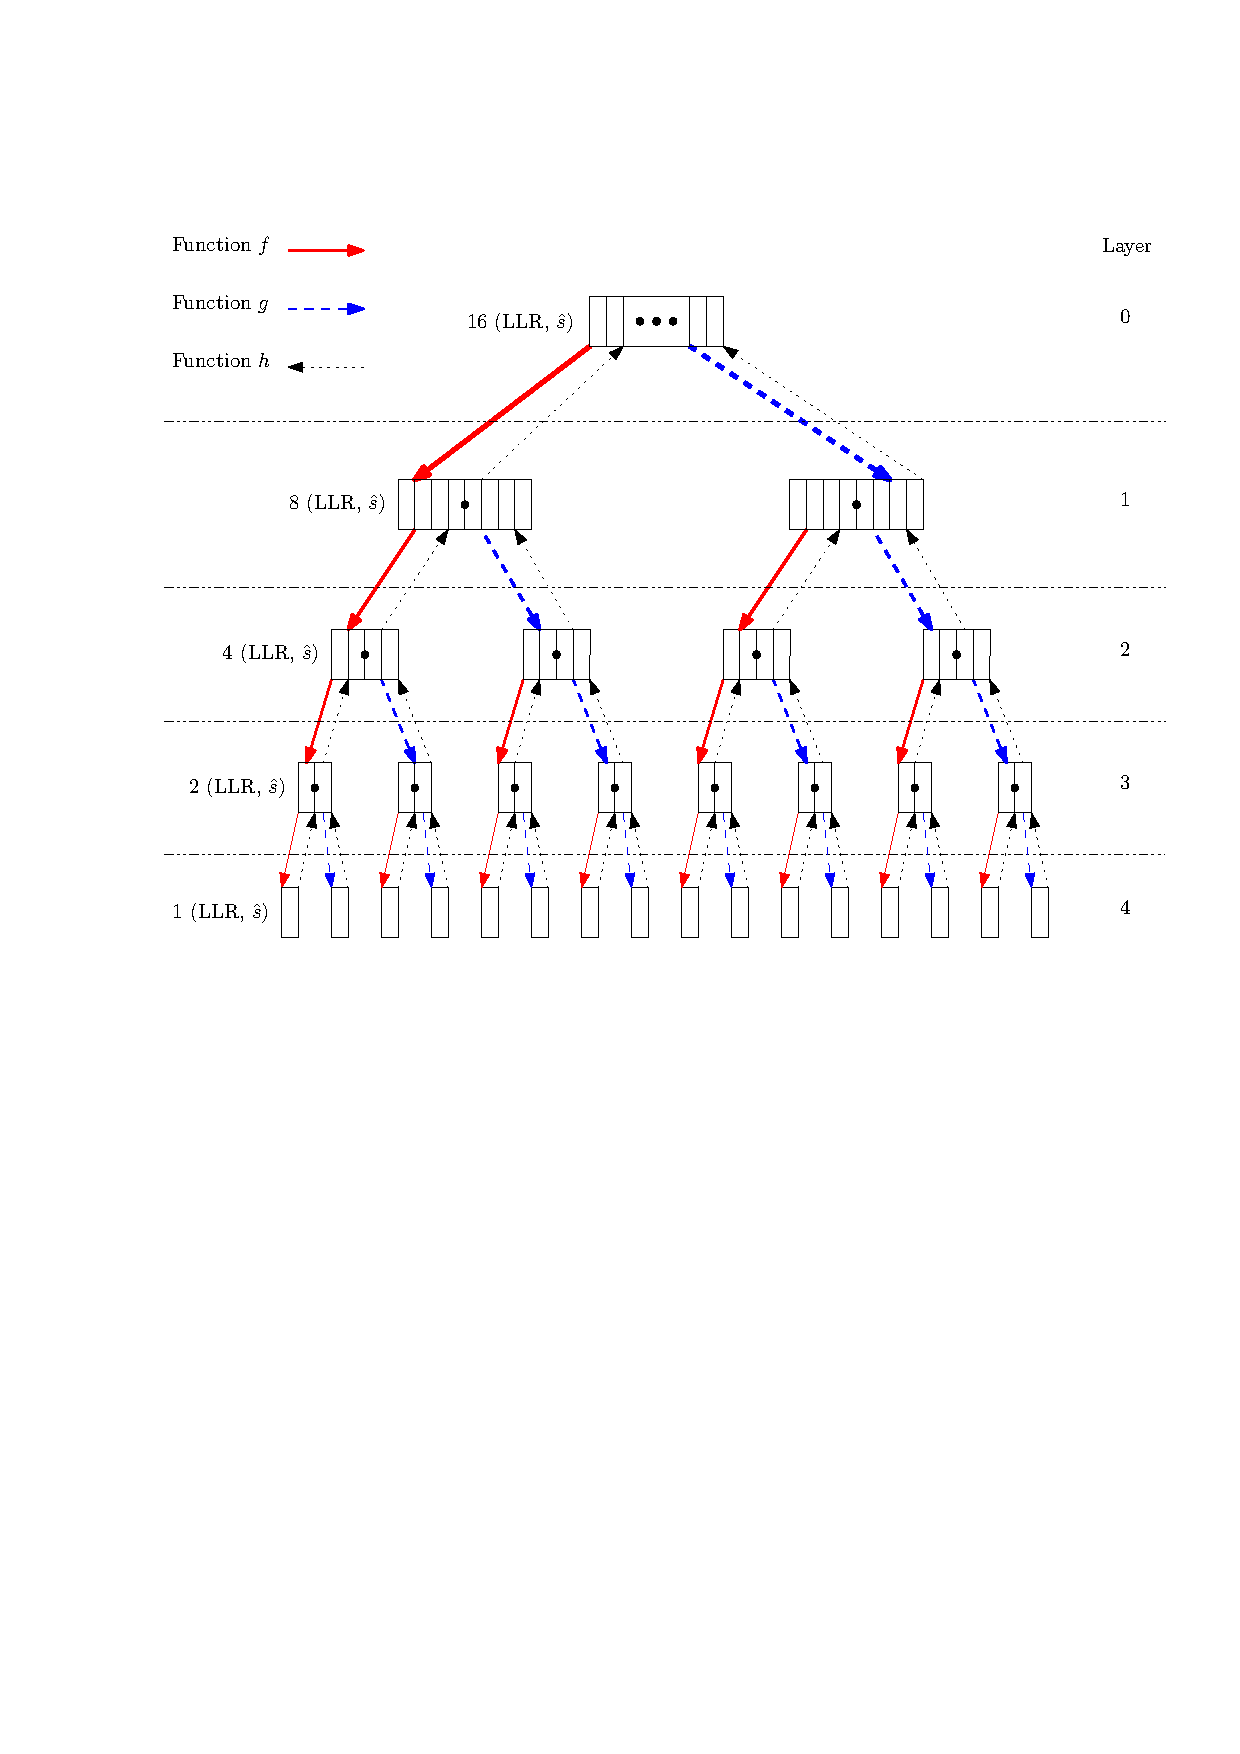
\includegraphics[width=0.70\textwidth]{polar/sc_decoder}
  \caption{Full SC decoding tree (N = 16)}
  \label{fig:polar_sc_decoder}
\end{figure}

The SC decoding algorithm can be seen as the traversal of a binary tree starting
from the root node. For a code length $N=2^m$, the corresponding tree thus
includes $m + 1$ node layers, indexed from $d=0$ (root node layer) down to
$d=m$ (leaf nodes layers). As the tree is initially full, each layer $d$
contains $2^d$ nodes, each node of that layer $d$  containing $2^{m-d}$ LLRs
($\lambda$) and $2^{m-d}$ binary values denoted as \textit{partial sums} ($s$).
At initialization, LLRs received  from the channel ($Y$) are stored in the root
node. Then, the decoder performs a pre-order traversal of the tree. When a node
is visited in the downward direction, LLRs of the node are updated. In the
upward direction, partial sums are updated. Fig.~\ref{fig:polar_sc_decoder}
summarizes the computations performed in both directions. The update functions
are:
\begin{eqnarray}
\left\{\begin{array}{l c l c l}
\lambda_c &=& f(\lambda_a,\lambda_b) &=& sign(\lambda_a.\lambda_b).\min(|\lambda_a|,|\lambda_b|)\\
\lambda_c &=& g(\lambda_a,\lambda_b,s)&=&(1-2s)\lambda_a+\lambda_b\\
(s_{c}, s_{d}) &=& h(s_{a}, s_{b}) &=& (s_{a} \oplus s_{b}, s_{b}).
\end{array}\right.
\label{eq:f_g}
\end{eqnarray}
The $f$ and $g$ functions both generate a single LLR. The $h$ function provides
a couple of partial sums.

Before recursively calling itself on the left node, the algorithm apply the $f$
function, respectively, before calling itself on the right node the $g$ function
is applied. At the end (after the recursive call on the right node) the $h$
function is applied. The $f$ and $g$ functions use the LLRs (read only mode)
from the current node $n_i$ in order to produce the new LLR values into
respectively left and right $n_{i+1}$ nodes. The $h$ function, in the general
case (non-terminal case), reads the bits from the left and right $n_{i+1}$ nodes
in order to update the bit values of the $n_i$ node. For the terminal case, the
$h$ function reads the LLRs from itself and decides the bit values.

Leaf nodes are of two kinds: \emph{information bit} nodes and \emph{frozen bit}
nodes. When a frozen bit leaf node is reached, its binary value is
unconditionally set to zero. Instead, when an information leaf node is reached,
its binary value is set according to the \emph{sign} of its LLR (0 if LLR is
positive, 1 otherwise). Once every node in the tree has been visited in both
directions, the decoder eventually updates partial sums in the root node and the
decoding process is terminated. At this point, the decoding result is stored in
the root node in the form of a $N$-bit partial sum vectors.

\subsubsection{Successive Cancellation List Algorithm}

\begin{algorithm}
  \caption{SCL decoding algorithm}\label{alg:polar_scl}

  \small
  \SetKwProg{Fn}{Function}{}{}

  % \KwIn{$N$ is the frame size.}
  % \KwIn{$L$ is the number of lists (or paths) to maintain.}
  \KwData{$\lambda$ is a 2D buffer ($[L][2N]$) to store the LLRs.}
  \KwData{$\hat{s}$ is a 2D buffer ($[L][N]$) to store the bits.}

  \Fn{SCL\_decode ($N, o_{\lambda}, o_{\hat{s}}$)}
  {
    $N_{\frac{1}{2}} = N / 2$

    \uIf(// not a leaf node){$N > 1$}
    {
      \For(// loop over the paths){$p=0$ \textbf{to} $L-1$}
      {
        \For(// apply the $f$ function){$i=0$ \textbf{to} $N_{\frac{1}{2}}-1$}
        {
          $\lambda[p][o_\lambda + N + i] = \bm{f}(\lambda[p][o_\lambda + i], \lambda[p][o_\lambda + N_{\frac{1}{2}} + i])$
        }
      }

      \textit{SCL\_decode ($N_{\frac{1}{2}}, o_{\lambda} + N, o_{\hat{s}}$)}

      \For{$p=0$ \textbf{to} $L-1$}
      {
        \For(// apply the $g$ function){$i=0$ \textbf{to} $N_{\frac{1}{2}}-1$}
        {
          $\lambda[p][o_\lambda + N + i] = \bm{g}(\lambda[p][o_\lambda + i], \lambda[p][o_\lambda + N_{\frac{1}{2}} + i], \hat{s}[p][o_{\hat{s}} + i])$
        }
      }

      \textit{SCL\_decode ($N_{\frac{1}{2}}, o_{\lambda} + N, o_{\hat{s}} + N_{\frac{1}{2}}$)}

      \For{$p=0$ \textbf{to} $L-1$}
      {
        \For(// update the partial sums){$i=0$ \textbf{to} $N_{\frac{1}{2}}-1$}
        {
          $\hat{s}[p][o_{\hat{s}} + i] = \bm{h}(\hat{s}[p][o_{\hat{s}} + i], \hat{s}[p][o_{\hat{s}} + N_{\frac{1}{2}} + i])$
        }
      }
    }
    \Else(// a leaf node)
    {
      \textit{update\_paths ()} // update, create and delete paths
    }
  }

  \textit{SCL\_decode ($N, 0, 0$)} // launch the decoder

  \textit{select\_best\_path ()}
\end{algorithm}

The SCL algorithm is summarized in Algorithm~\ref{alg:polar_scl}. Unlike the SC
algorithm, the SCL decoder builds a list of candidate codewords along the
decoding. At each call of the \textit{update\_paths()} sub-routine
(Alg.~\ref{alg:polar_scl}, l.16), $2L$ candidates are generated. A path metric
is then evaluated to keep only the $L$ best candidates among the $2L$ paths. The
path metrics are calculated as in \cite{Balatsoukas-Stimming2015}. At the end of
the decoding process, the candidate codeword with the best path metric is
selected in the \textit{select\_best\_path()} sub-routine
(Alg.~\ref{alg:polar_scl}, l.18). The decoding complexity of the SCL algorithm
grows as $O(LN\log_2N)$. This linear increase in complexity with L leads to
significant improvements in BER/FER performances, especially for small code
lengths.

\paragraph{CRC concatenation scheme}

The authors in~\cite{Tal2011} observed that when a decoding error occurs, the
right codeword is often in the final list, but not with the best path metric.
They proposed to concatenate a CRC to the codeword in order to discriminate the
candidate codewords at the final stage of the SCL decoding. Indeed, this
technique drastically improves the FER performance of the decoder. We denote
this algorithm CA-SCL and its simplified version CA-SSCL. In terms of
computational complexity, the overhead consists in the computation of $L$ CRC at
the end of each decoding.

\paragraph{Adaptive SCL decoding algorithm}

The presence of the CRC can be further used to reduce the decoding time by
gradually increasing $L$. This variation of SCL is called Adaptive SCL
(A-SCL)~\cite{Li2012}. The first step of the A-SCL algorithm is to decode the
received frame with the SC algorithm. Then, the decoded polar codeword is
checked with a CRC. If the CRC is not valid, the SCL algorithm is applied with
$L=2$. If no candidate in the list satisfies the CRC, $L$ is gradually doubled
until it reaches the value $L_{max}$. In this paper, we call this version of the
A-SCL decoding the Fully Adaptive SCL (FA-SCL) as opposed to the Partially
Adaptive SCL (PA-SCL), in which the $L$ value is not gradually doubled but
directly increased from $1$ (SC) to $L_{max}$. The simplified versions of these
algorithms are denoted PA-SSCL and FA-SSCL. In order to simplify the algorithmic
range, in the remainder of the paper, only the simplified versions are
considered. The use of either FA-SSCL or PA-SSCL algorithmic improvement
introduces no BER or FER performance degradation as long as the CRC length is
adapted to the polar code length. If the CRC length is too short, the decoding
performance may be degraded because of false detections. These adaptive versions
of SSCL can achieve higher throughputs. Indeed, a large proportion of frames can
be decoded with a single SC decoding. This is especially true when the SNR is
high. This will be further discussed in Section~\ref{sec:genericity}.

\subsubsection{Optimization Strategies}

\begin{itemize}
  \item \cmark~polar API
  \item \cmark~inter/intra-SIMD
  \item \cmark~élagage
  \item \cmark~déroulage des appels récursifs
\end{itemize}

The previous decoder algorithms has a number of characteristics of interest for
its optimization. Generating decoders able to take advantage of this
optimization space is the key for high performance decoders:
\begin{itemize}
  \item The tree traversal is sequential, but $f$, $g$ and $h$ are applied
    element-wise to all elements of the LLR and bits in the nodes and
    their children. As there is no dependence between computations
    involving different elements of the same node, these node computations
    can be parallelized or vectorized (cf. the \emph{intra-frame} strategy
    introduced in~\cite{Giard2014}),
  \item Frozen bits fully define their leaf values, hence some part of the
    traversal can be cut and its computation avoided, depending on the
    location of the frozen bits. More generally, the tree computation can
    be versioned depending on these bits. In~\cite{Alamdar-Yazdi2011}, a tree
    pruning technique called the Simplified SC (SSC) was applied to SC decoding.
    An improved version was proposed in~\cite{Sarkis2014a}. This technique
    relies on the fact that, depending on the frozen bits location in the leaves
    of the tree, the definition of dedicated nodes enables to prune the decoding
    tree: Rate-0 nodes (\texttt{R0}) correspond to a sub-tree whose all leaves
    are frozen bits, Rate-1 nodes (\texttt{R1}) correspond to a sub-tree in
    which all leaves are information bits, REPetition (\texttt{REP}) and Single
    Parity Check (\texttt{SPC}) nodes correspond to repetition and SPC codes
    sub-trees. These special nodes, originally defined for SC decoding, can be
    employed in the case of SCL decoding as long as some modifications are made
    in the path metric calculation~\cite{Sarkis2016}. This tree-pruned version
    of the algorithm is called Simplified SCL (SSCL). The tree pruning technique
    can drastically reduce the amount of computation in the decoding process,
  \item The decoder can be specialized for a particular configuration of frozen
    bits, as frozen bit locations do not change for many frames,
  \item Similarly, multiple frames can be decoded concurrently, with parallel or
    vector code. Such \emph{inter-frame} optimizations can increase the decoding
    throughput, however at the expense of latency, which is also one important
    metric of the application (cf.~\cite{LeGal2015a}).
\end{itemize}

Beside optimizations coming from the computations in the tree, several
representations of LLR may lead to different error correction performance. LLR
for instance can be represented by floats or integers (fixed point
representation), LLR from different frames can be packed together.

Finally, usual code optimizations, such as unrolling or inlining can also be
explored. For instance, the recursive structure of the tree computation can be
fully flatten, depending on the size of the code length.

\subsubsection{Algorithmic Comparison}

\begin{table}
  \centering
  \caption{Throughput and latency comparison of polar decoding algorithms.}
  \label{tab:polar_algos}
  {\small
   \begin{tabular}{r|c|c|c}
    \textbf{Decoding}  & \textbf{BER \& FER}   & \multirow{1}{*}{\textbf{Throughput}} & \textbf{Max. Latency}        \\
    \textbf{Algorithm} & \textbf{Performances} & ($\bm{\mathcal{T}}$)                 & ($\bm{\mathcal{L}_{worst}}$) \\
    \hline
    SC      & poor      & medium & medium \\
    SSC     & poor      & high   & low    \\
    SCL     & good      & low    & high   \\
    SSCL    & good      & low    & medium \\
    CA-SSCL & very good & low    & medium \\
    PA-SSCL & very good & high   & medium \\
    FA-SSCL & very good & high   & high   \\
  \end{tabular}
  }
\end{table}

In order to better distinguish all the algorithmic variations, we compare their
main features in Table~\ref{tab:polar_algos}. Each algorithm is characterized in
terms of decoding performance, throughput, and worst case latency for a software
implementation. The non-simplified versions of the adaptive SCL algorithms are
not included in the Table for readability.

The SC and especially the SSC algorithms achieve very high throughput and low
latency with poor BER and FER performances. The SCL algorithm improves the
decoding performance compared to the SC algorithm, but its computational
complexity leads to an increased latency and a lower throughput. The SSCL
algorithm improves the decoding throughput and latency without any impact in
terms of BER and FER performances, as long as the tree pruning is not too deep,
as will be discussed in Section~\ref{sec:genericity}. Therefore, tree pruning is
applied to all the following algorithms, namely CA-SSCL, FA-SSCL and PA-SSCL. By
applying CRC to the SCL algorithm, one can achieve better BER and FER
performances at the cost of computational complexity overhead. The Adaptive SCL
algorithms reduce the decoding time with no impact on BER and FER performances.
Furthermore, a tradeoff between throughput and worst case latency is possible
with the use of either PA-SSCL or FA-SSCL decoding algorithms.

\begin{figure}
  \centering
  \includegraphics[width=0.7\textwidth]{polar/algos_comparison/algos_comparison}
  \caption{Decoding performance comparison between CA-SCL and SC decoders.
    Code rate $R = 1/2$, and 32-bit CRC (GZip).}
  \label{plot:polar_algos_comparison}
\end{figure}

CA-SCL decoding performances for large code lengths ($N > 2^{14}$) combined with
large list sizes ($L > 8$) are rarely presented in the literature. This is
probably due to the long simulation time. The proposed decoders are integrated
in the AFF3CT toolbox. Therefore, multi-threaded and multi-nodes simulations
are enabled to handle such computation-demanding simulations. All the presented
simulations use the Monte Carlo method with a Binary Phase-Shift Keying (BPSK)
modulation. The communication channel is an Additive White Gaussian Noise (AWGN)
channel based on the Mersenne Twister pseudo-random number generator
(MT19937)~\cite{Matsumoto1998} and the Box-Muller transform~\cite{Box1958}.
Figure~\ref{plot:polar_algos_comparison} compares the BER/FER performances of
CA-SCL with SC decoding for a large range of code lengths. As expected, it
appears that the coding gain brought by the SCL algorithm decreases for larger
$N$ values. In the case of $N=2^{16}$, the improvement caused by the use of the
CA-SCL algorithm with $L=32$ and a 32-bit GZip CRC (\texttt{0x04C11DB7}
polynomial) instead of SC is about $0.75$ dB compared to $1.2$ dB with a polar
code of size $N=2^{12}$. For larger polar codes, $N=2^{20}$, the gain is reduced
to $0.5$ dB, even with a list depth of $128$ that is very costly in terms of
computational complexity.

The tradeoffs between speed and decoding performance show some general trends.
However, the efficiency of each decoding algorithm is strongly dependent on the
polar code length, code rate, list depth and code construction. It is expected
that the best tradeoff is not always obtained with a single algorithm and
parameter set combination. It is consequently highly relevant to use a generic
and flexible decoder, that supports all variants of the decoding algorithms.
Thus, it is possible to switch from one to another as shown in the following
section.

\subsubsection{Generic and Flexible Polar Decoders}
\label{sec:genericity}

The main contribution of this work lies in the flexibility and the genericity of
the proposed software decoder. These terms need to be clearly defined in order
to circumvent possible ambiguity. In the remainder of the paper, the
\textit{genericity} of the decoder concerns all the parameters that define the
supported polar code such as the codeword length, the code rate, the frozen bits
set, the puncturing patterns and the concatenated CRC. These parameters are
imposed by the telecommunication standard or the communication context. In the
wireless communications context, these are constantly adapted by AMC
methods~\cite{Dahlman2013}. In this work, a decoder is considered
\textit{generic} if it is able to support any combination of these parameters
that can be changed during a real time execution. On the other hand, the
\textit{flexibility} of a decoder includes all the customizations that can be
applied to the decoding algorithm for a given polar code: variant of the
decoding algorithm, data quantization, list size $L$, tree pruning strategy, ...
These customizations are not enforced by a standard. The flexibility gives some
degrees of freedom to the decoder in order to find the best tradeoff between
decoding performance, throughput or latency for a given polar code.

\paragraph{Genericity}

In the context of wireless communications, the standards enforce several
different code lengths $N$ that have to be supported to share bandwidth between
different users. This is also the case for the code rate $R$ that needs to be
adapted to the quality of the transmission channel. Therefore, a practical
implementation should be adapted to both $N$ and $R$ in real-time in order to
limit latency.

A polar code is completely defined by $N$ and the frozen bits set
$\bm{u}_{\mathcal{A}^c}$. Several methods exist to generate some "good" sets of
frozen bits~\cite{Tal2013,Trifonov2012}. The code rate $R$ depends on the size
of $\bm{u}_{\mathcal{A}^c}$. In their original form, polar code lengths are only
powers of two. The puncturing and shortening techniques
in~\cite{Wang2014,Niu2013,Miloslavskaya2015} enable to construct polar codes of
any length at the cost of slightly degraded decoding performance. The coding
scheme can be completed with the specification of a CRC.

In~\cite{Sarkis2016}, the unrolling method is used: a specific description of
the decoder has to be generated for a specific polar code parameter set of $N$,
$K$, $R$, frozen bits set, puncturing pattern, CRC. This approach leads to very
fast software decoders at the price of the genericity, since a new source code
should be generated and compiled every time the modulation and coding scheme
(MCS) changes. This method is not adapted to wireless communication standards,
in which these parameters have to be adapted not only over time, but also for
the different users.

The proposed decoder does not use the unrolling method and is completely generic
regarding the code dimension $K$, the code length $N$, the frozen bits set
$\bm{u}_{\mathcal{A}^c}$ and the puncturing patterns. All of them are dynamic
parameters of the decoder and can be defined in input files. All CRC listed
in~\cite{CRCWiki2017} are available along with the possibility to define others.
It is shown in~\cite{Zhang2017} that custom CRCs for polar codes can have a very
good impact on the decoding performance.

Relying on an unique software description also implies that the tree pruning
technique also has to be dynamically defined. Indeed, this technique depends on
the frozen bits set $\bm{u}_{\mathcal{A}^c}$. Not sacrificing throughput or
latency while maintaining the genericity imposed by wireless communication
standards is at the core of the proposed implementation. Flexibility in terms of
decoding algorithms, described in the following, along with improvements
presented in Section~\ref{sec:implem_improv}, is necessary to deal with this
challenge.

\paragraph{Flexibility}

On one hand, the reason for the decoder genericity is the compliance to the
telecommunication standards. On the other hand, the flexibility of the decoder
regroups several algorithmic variations that are discussed in the following.
These variations allow several tradeoffs of multiple sorts, whatever the
standard. They are all included in a single source code.

In the proposed decoders the following parameters can be changed dynamically
without re-compilation: the list size $L$, the tree pruning strategy, the
quantization of the LLRs and the different SCL variants. Each of these
adjustments can be applied to access to different tradeoffs between throughput,
latency, and error rate performance. As a consequence, one can easily fine-tune
the configuration of the software decoder for any given polar code.

\subparagraph{List size}

\begin{figure}
  \centering
  \includegraphics[width=0.70\textwidth]{polar/scl_l/scl_l}
  \caption{Tradeoffs between CA-SSCL decoding and throughput performances
    depending on $L$. $N=2048$, $R=0.5$, and 32-bit CRC (GZip). For $L=1$, the
    SSC decoder is used with a ($2048$,$1024$) polar code.}
  \label{plot:polar_scl_l}
\end{figure}

As mentioned earlier, the list size $L$ impacts both speed and decoding
performance. In Figure~\ref{plot:polar_scl_l}, the throughput as well as BER and
FER performances of the CA-SSCL algorithm are shown for different $L$ values. A
($2048$,$1024$) polar code with a 32-bit CRC is considered. The computational
complexity increases linearly with $L$: the throughput is approximately halved
when $L$ is doubled, except for the case of the SC algorithm ($L=1$) which is
much faster. Indeed, there is no overhead due to the management of different
candidate paths during the decoding. For $L\geq4$ and $E_b/N_0=2$, the FER is
also approximately halved when the list size $L$ is doubled.

\subparagraph{Tree pruning strategy}

% SC --------------------------------------------------------------------------
\begin{figure}[htp]
\includegraphics[width=1.00\textwidth]{polar/sc_tree_cut/sc_tree_cut}
\caption{Throughput depending on the different optimizations for $N = 2048$, for
  intra-frame vectorization on the left and intra-frame vectorization on the
  right, resp. (on the Intel Xeon CPU E31225).}
\label{plot:polar_sc_tree_cut}
\end{figure}

The tree pruning step has a dramatical effect in general. For example, the
reference code for a rate of 1/2 has 2047 nodes, whereas only 291 nodes remain
in the pruned version. However, the individual effect of each rewriting rule is
not trivial. The plots in Fig.~\ref{plot:polar_sc_tree_cut} show the respective
impact of several rewriting rules (cuts, repetitions, single parity checks
(SPC)), with $N = 2048$ and multiple code rates, for Intra-SIMD and Inter-SIMD
respectively. The purpose of the plots is to show that no single rewriting rule
dominates for every code rate, and that the respective impact of each rule may
vary a lot from rate to rate, making the case for the flexible, extensible
architecture of P-EDGE. Indeed, P-EDGE's rewriting rule set can also be enriched
with rules for specific ranges of code rate. For instance, the rule
\emph{Single Parity Check (SPC)} has been applied with different level limits
for 9/10 code rate, where it has a significant impact and may benefit from fine
tuning.

% SCL -------------------------------------------------------------------------
\begin{figure}
  \centering
  \includegraphics[width=0.70\textwidth]{polar/scl_tree_cut/scl_tree_cut}
  \caption{Impact of the specialized nodes on the SCL coded throughput.
  % \caption{Dedicated nodes impact on CA-SSCL.
    $N=2048$ and $L=32$.}
  \label{plot:polar_scl_tree_cut}
\end{figure}

A second degree of flexibility is the customization of the SCL tree pruning. The
authors in~\cite{Alamdar-Yazdi2011,Sarkis2016} defined dedicated nodes to prune
the decoding tree and therefore to reduce the computational complexity. In this
proposed decoder, each dedicated node can be activated separately. The ability
to activate dedicated nodes at will is useful in order to explore the
contribution of each node type on the throughput.
Figure~\ref{plot:polar_scl_tree_cut} shows the impact of the different tree
pruning optimizations on the CA-SSCL decoder throughput depending on the code
rate. The performance improvements are cumulative. Coded throughput, in which
the redundant bits are taken in account, is shown instead of information
throughput, for which only information bits are considered in order to
illustrate the computational effort without the influence of the fact that
higher rate codes involve higher information throughput.

The coded throughput of the original unpruned algorithm (\texttt{ref}),
decreases as the code rate increases. Indeed, frozen bit leaf nodes are faster
to process than information bit leaf nodes, in which a threshold detection is
necessary. As there are more \texttt{R0} and \texttt{REP} nodes in low code
rates, the tree pruning is more efficient in the case of low code rates. The
same explanation can be given for \texttt{R1} nodes in high code rates.
\texttt{R1} node pruning is more efficient than \texttt{R0} node pruning on
average. Indeed, a higher amount of computations is saved in \texttt{R1} nodes
than in \texttt{R0} nodes.

It has also been observed in~\cite{Sarkis2016} that when the \texttt{SPC} node
size is not limited to $4$, the decoding performance may be degraded.
Consequently the size is limited to $4$ in \texttt{SPC4}. In \texttt{SPC4+}
nodes, there is no size limit. The two node types are considered in
Figure~\ref{plot:polar_scl_tree_cut}. Therefore, the depth at which dedicated
nodes are activated in the proposed decoder can be adjusted, in order to offer a
tradeoff between throughput and decoding performance.

\begin{figure}
  \centering
  \includegraphics[width=0.70\textwidth]{polar/scl_spc/scl_spc_diff}
  % \caption{Impact of the specialized nodes on the SCL coded throughput.
  \caption{Effects of the \texttt{SPC4+} nodes on the CA-SSCL @ $10^{-5}$ FER}
  \label{fig:polar_scl_spc}
\end{figure}

According to our experiments, the aforementioned statement about performance
degradation caused by \texttt{SPC4+} nodes is not always accurate depending on
the code and decoder parameters. The impact of switching \textit{on} or
\textit{off} \texttt{SPC4+} nodes on decoding performance and throughput at a
FER of $10^{-5}$ is detailed in Figure~\ref{fig:polar_scl_spc}. It shows that
\texttt{SPC4+} nodes have only a small effect on the decoding performance. With
$L=8$, an SNR degradation lower than 0.1 dB is observed, except for one
particular configuration. Throughput improvements of $8$ to $23$ percents are
observed. If $L=32$, the SNR losses are more substantial (up to $0.5$ dB),
whereas throughput improvements are approximately the same. Besides this
observation, Figure~\ref{fig:polar_scl_spc} shows how the proposed decoder
flexibility in the AFF3CT environment enables to optimize easily the decoder
tree pruning, both for software implementations or for hardware implementations
in which tree pruning can also be applied~\cite{Lin2014}.

\subparagraph{LLR Quantization}

\begin{figure}
  \centering
  \includegraphics[width=0.70\textwidth]{polar/scl_bfer/scl_bfer}
  \caption{Decoding performance of the SSCL and the A-SSCL decoders.
    Code ($2048$,$1723$), $L=32$.}
  \label{plot:polar_scl_bfer}
\end{figure}

\begin{table}
  %\renewcommand{\arraystretch}{1.1}
  \centering
  \caption{Throughput and latency comparisons between floating-point (32-bit)
    and fixed-point (16-bit and 8-bit) Adaptive SSCL decoders. Code (2048,1723),
    $L = 32$ and 32-bit CRC (Gzip).}
  \label{tab:polar_scl_perfs_fixed}
  %{\small\resizebox{\linewidth}{!}{
  \begin{tabular}{r | r | c || c | c || c | c || c | c}
    \multirow{2}{*}{\textbf{Decoder}} & \multirow{2}{*}{\textbf{Prec.}} & \multirow{2}{*}{$\bm{\mathcal{L}_{worst}}$} & \multicolumn{2}{c ||}{\textbf{3.5 dB}} & \multicolumn{2}{c ||}{\textbf{4.0 dB}} & \multicolumn{2}{c}{\textbf{4.5 dB}} \\
    \cline{4-9}
    & & & $\bm{\mathcal{L}_{avg}}$ & $\bm{\mathcal{T}_i}$ & $\bm{\mathcal{L}_{avg}}$ & $\bm{\mathcal{T}_i}$ & $\bm{\mathcal{L}_{avg}}$ & $\bm{\mathcal{T}_i}$ \\
    % \hline
    \hline
    \multirow{3}{*}{PA-SSCL} & 32-bit &  635 & 232.3 &   7.6 & 41.7 &  42.1 & 7.4 & 237.6 \\
    %\cline{3-9}
                             & 16-bit &  622 & 219.6 &   8.0 & 40.1 &  43.8 & 6.6 & 267.5 \\
    %\cline{3-9}
                             &  8-bit &  651 & 232.4 &   7.6 & 41.2 &  42.6 & 6.5 & 268.3 \\
    \hline
    \multirow{3}{*}{FA-SSCL} & 32-bit & 1201 &  67.2 &  26.1 &  8.5 & 207.8 & 5.1 & 345.5 \\
    %\cline{3-9}
                             & 16-bit & 1198 &  68.7 &  25.6 &  7.7 & 225.7 & 4.3 & 408.7 \\
    %\cline{3-9}
                             &  8-bit & 1259 &  71.8 &  24.4 &  7.7 & 227.3 & 4.1 & 425.9 \\
  \end{tabular}
  %}}
\end{table}

Another important parameter in both software and hardware implementations is the
quantization of data in the decoder. More specifically, the quantization of LLRs
and partial sums in the decoder have an impact on decoding performance.
Quantized implementations of the SC algorithm have already been proposed
in~\cite{Giard2016} but to the best of our knowledge, the proposed decoder is
the first SCL software implementation that can benefit from the 8-bit and 16-bit
fixed-point representations of LLRs and internal path metrics. In the 8-bit mode
LLRs and path metrics are saturated between $-127$ and $+127$ after each
operation. Moreover, to avoid overflows, the path metrics are normalized after
each \textit{update\_paths()} call (cf. Alg.~\ref{alg:polar_scl}) by subtracting
the smallest metric to each one of them. Figure~\ref{plot:polar_scl_bfer}a shows
the BER and FER performances of the CA-SSCL decoder for 32-bit floating-point,
16-bit and 8-bit fixed-point representations. One can observe that the
\texttt{REP} nodes degrade the decoding performance in a 8-bit representation
because of accumulation (red triangles curve). Indeed, it is necessary to add
all the LLRs of a \texttt{REP} node together in order to process it, which may
lead to an overflow in the case of fixed-point representation. It can happen
when the size of the repetition nodes is not limited
($\texttt{REP}_\texttt{2+}$). However, the size limitation of the repetition
nodes to 8 ($\texttt{REP}_\texttt{8-}$) fixes this issue. In
Table~\ref{tab:polar_scl_perfs_fixed}, maximum latency ($\mathcal{L}_{worst}$ in
$\mu s$), average latency ($\mathcal{L}_{avg}$ in $\mu s$) and information
throughput ($\mathcal{T}_i$ in Mb/s) are given. Note that in 8-bit configuration
only the \texttt{REP}$_{\texttt{8-}}$ nodes are used. The fixed-point
implementation reduces, on average, the latency. In the high SNR region, the
frame errors are less frequent. Therefore, the SCL algorithm is less necessary
than in low SNR regions for Adaptive SCL algorithms. As the gain of fixed-point
implementation benefits more to the SC algorithm than to the SCL algorithm, the
throughput is higher in high SNR regions. For instance, up to 425.9 Mb/s is
achieved in 8-bit representation with the FA-SSCL decoder. Note that the
improvements described in Section~\ref{sec:implem_improv} are applied to the
decoders that are given in Table~\ref{tab:polar_scl_perfs_fixed}.

\subparagraph{Supporting different variants of the decoding algorithms}

Besides the $L$ values, the tree pruning and quantization aspects, the proposed
software polar decoder supports different variants of the SCL algorithm:
CA-SSCL, PA-SSCL, FA-SSCL.

\begin{figure}
  \centering
  \includegraphics[width=0.70\textwidth]{polar/scl_adaptive/scl_adaptive}
  \caption{Frame Error Rate (FER) performance and throughput of the Fully and
    Partially Adaptive SSCL decoders (FA and PA). Code ($2048$,$1723$) and
    32-bit CRC (GZip). 32-bit floating-point representation.}
  \label{plot:polar_scl_adaptive}
\end{figure}

As shown in~\cite{Sarkis2016}, the adaptive version of the SCL algorithm yields
significant speedups, specially for high SNR. The original adaptive SCL
described in~\cite{Li2012}, denoted as Fully Adaptive SCL (FA-SSCL) in this
paper, gradually doubles the list depth $L$ of the SCL decoder when the CRC is
not valid for any of the generated codewords at a given stage until the value
$L_{max}$. By contrast, the adaptive decoding algorithm implemented
in~\cite{Sarkis2016}, called in this paper Partially Adaptive SCL (PA-SSCL),
directly increases the list depth from $1$ (SC) to $L_{max}$. In
Figure~\ref{plot:polar_scl_adaptive}, the two versions (FA-SSCL and PA-SSCL) are
compared on a ($2048$,$1723$) polar code and 32-bit CRC (GZip). The LLRs values
are based on a 32-bit floating point representation. Note that as the FER
performance of PA-SSCL and FA-SSCL are exactly the same, the related error
performance plots completely overlap. The throughput of the FA-SSCL algorithm is
higher than that of the PA-SSCL algorithm for some SNR values, depending on the
code parameters. Considering typical FER values for wireless communication
standards ($10^{-3}$ to $10^{-5}$), in the case of a ($2048$,$1723$) polar code,
the throughput of FA-SSCL is double that of PA-SSCL with $L = 8$, while it is
multiplied by a factor of $7$ with $L=32$. The drawback of FA-SSCL is that
although the average latency decreases, the worst case latency increases.

The adaptive versions of the algorithm achieve better throughputs, but CA-SCL
may also be chosen depending on the CRC. One may observe in
Figure~\ref{plot:polar_scl_bfer}b that an adaptive decoder dedicated to an 8-bit
CRC with a ($2048$,$1723$) polar code and $L=32$ leads to a loss of $0.5$ dB for
a FER of $10^{-5}$ compared to its non adaptive counterpart.

Both polar code genericity and decoding algorithm flexibility are helpful to
support the recommendations of wireless communications in an SDR or cloud RAN
context. The code and decoder parameters can be dynamically changed in the
proposed decoder, while maintaining competitive throughput and latency. The
following section introduces algorithmic and implementation improvements applied
in the proposed decoders to keep a low decoding time.

\paragraph{Software implementation optimizations}
\label{sec:implem_improv}

The genericity and flexibility of the formerly described decoder prevent from
using some optimizations. Unrolling the description as in~\cite{Sarkis2016} is
not possible at runtime, although code generation could be used to produce an
unrolled version of any decoder as in \cite{Cassagne2015c}. Moreover, in the
case of large code lengths, the unrolling strategy can generate very large
compiled binary files. This can cause instruction cache misses that would
dramatically impact the decoder throughput. On the contrary, the size of the
executable files of the proposed decoder are constant with respect to the code
parameters (N, L, K). The number of cycles lost due to cache misses is,
according to our experiments, less than 0.01\% of the total number of cycles.
Still, some implementation improvements are necessary in order to be competitive
with specific unrolled decoders of the literature. The software library for
polar codes from \cite{Cassagne2015c,Cassagne2016b} enables to benefit from
the SIMD instructions for various target architectures. Optimizations of CRC
checking benefit to both the non-adaptive and adaptive versions of the CA-SCL
algorithms. The new sorting technique presented in Section~\ref{subsec:sorting}
can be applied to each variation of the SCL algorithm. Finally, an efficient
implementation of the partial sums memory management is proposed. It is
particularly effective for short polar codes.

\subparagraph{Polar Application Programming Interface}

\begin{listing}
  \inputminted[frame=lines,linenos]{C++}{main/chapter2/src/polar/f_g_h_simd.cpp}
  \caption{C++ SIMD implementation of the $f$, $g$ and $h$ functions.}
  \label{lst:polar_f_g_h_simd}
\end{listing}

Reducing the decoding time with SIMD instructions is a classical technique in
former software polar decoder implementations. The proposed list decoders are
based on specific building blocks included from the Polar
API~\cite{Cassagne2015c,Cassagne2016b}. These blocks are fast and optimized
implementations of the $f$, $g$, $h$ (and their variants) polar intrinsic
functions. Listing~\ref{lst:polar_f_g_h_simd} details the SIMD implementation of
these  functions. This implementation is based on MIPP, a SIMD wrapper for the
intrinsic functions (assembly code), and the template meta-programming
technique. Consequently, the description is clear, portable, multi-format
(32-bit floating-point, 16-bit and 8-bit fixed-points) and as fast as an
architecture specific code. The \texttt{mipp::Reg<B>} and \texttt{mipp::Reg<R>}
types correspond to SIMD registers. \texttt{B} and \texttt{R} define the type of
the elements that are contained in this register. \texttt{B} for \textit{bit}
could be \texttt{int}, \texttt{short} or \texttt{char}. \texttt{R} for
\textit{real} could be \texttt{float}, \texttt{short} or \texttt{char}. In
Listing~\ref{lst:polar_f_g_h_simd}, each operation is made on multiple elements
at the same  time. For instance, line 22, the addition between all the elements
of the \texttt{neg\_la} and \texttt{lb} registers is executed in one CPU cycle.

In the context of software decoders, there are two well-known strategies to
exploit SIMD instructions: use the elements of a register to compute 1) many
frames in parallel (INTER frame) or 2) multiple elements from a single frame
(INTRA frame). In this paper, only the INTRA frame strategy is considered. The
advantage of this strategy is the latency reduction by comparison to the INTER
frame strategy. However, due to the nature of the polar codes, there are
sometimes not enough elements to fill the SIMD registers completely. This is
especially true in the nodes near the leaves. For this reason, SIMD instructions
in the lower layers of the tree do not bring any speedup. In this context, the
building blocks of the Polar API automatically switch from SIMD to sequential
implementations. In the case of the CA-SSCL algorithm, using SIMD instructions
for decoding a ($2048$, $1723$) polar code leads to an improvement of $20\%$ of
the decoding throughput on average for different values of the list depth $L$.

\subparagraph{Improving Cyclic Redundancy Checking}
\label{subsec:crc_improv}

By profiling the Adaptive SCL decoder, one may observe that a significant amount
of time is spent to process the cyclic redundancy checks. Its computational
complexity is O($LN$) versus the computational complexity of the SCL decoding,
O($LN\log N$). The first is not negligible compared to the second.

In the adaptive decoder, the CRC verification is performed a first time after
the SC decoding. In the following, we show how to reduce the computational
complexity of these CRC verifications.

First, an efficient CRC checking code has been implemented. Whenever the decoder
needs to check the CRC, the bits are packed and then computed 32 by 32. In order
to further speed up the implementation, a lookup table used to store
pre-computed CRC sub-sequences, and thus reduce the computational complexity.
The size of the lookup table is 1 KB.

After a regular SC decoding, a decision vector of size $N$ is produced. Then,
the $K$ information bits must be extracted to apply cyclic redundancy check. The
profiling of our decoder description shows that this extraction takes a
significant amount of time compared to the check operation itself. Consequently,
a specific extraction function was implemented. This function takes advantage of
the leaf node type knowledge to perform efficient multi-element copies.

Concerning SCL decoding, it is possible to sort the candidates according to
their respective metrics and then to check the CRC of each candidate from the
best to the worst. Once a candidate with a valid CRC is found, it is chosen as
the decision. This method is strictly equivalent to do the cyclic redundancy
check of each candidate and then to select the one with the best metric. With
the adopted order, decoding time is saved by reducing the average number of
checked candidates.

\subparagraph{LLR and Metric Sorting}
\label{subsec:sorting}

Metric sorting is involved in the aforementioned path selection step, but also
in the \textit{update\_paths()} sub-routine (Alg.~\ref{alg:polar_scl}, l.16) and
consequently in each leaf. Sorting the LLRs is also necessary in \texttt{R1} and
\texttt{SPC} nodes. Because of a lack of information about the sorting technique
presented in~\cite{Sarkis2016}, its reproduction is not possible. In the
following of the paragraph the sorting algorithm used in the SCL decoder is
described.

In \texttt{R1} nodes, a Chase-$2$~\cite{Chase1972} algorithm is applied. The two
minimum absolute values of the LLRs have to be identified. The way to do the
minimum number of comparisons to identify the $2$ largest of $n\geq2$ elements
was originally described by Schreier in~\cite{Schreier1932} and reported
in~\cite{Knuth1973}. The lower stages of this algorithm can be parallelized
thanks to SIMD instructions in the way described in~\cite{Furtak2007}. According
to our experimentations, Schreier's algorithm is the most efficient compared to
parallelized Batcher's merge exchange, partial quick-sort or heap-sort
implemented in the C++ standard library in the case of \texttt{R1} nodes. At the
end, we chose not to apply the SIMD implementation of the Schreier's algorithm
because: 1) the speedup was negligible, 2) in 8-bit fixed-point, only
$N \leq 256$ codewords can be considered.

Concerning path metrics, partial quick-sort appeared to yield no gains in terms
of throughput by comparison with the algorithm in~\cite{Schreier1932}, neither
did heap-sort or parallelized Batcher's merge exchange. For a matter of
consistency, only Schreier's algorithm is used in the proposed decoder, for both
LLR sorting in \texttt{R1} and \texttt{SPC} nodes and for path metrics sorting.
The sorting of path metrics is applied to choose the paths to be removed, kept
or duplicated.

\subparagraph{Partial Sum Memory Management}

An SCL decoder can be seen as $L$ replications of an SC decoder. The first
possible memory layout is the one given in Figure~\ref{fig:polar_sc_decoder}. In
this layout, the partial sums $\hat{s}$ of each node is stored in a dedicated
array. Therefore, a memory of size $2N-1$ bits is necessary in the SC decoder,
or $L(2N -1)$ bits in the SCL decoder. This memory layout is described
in~\cite{Tal2011} and applied in previous software
implementations~\cite{Sarkis2014b,Sarkis2016,Shen2016}.

A possible improvement is to change the memory layout to reduce its footprint.
Due to the order of operations in both SC and SCL algorithms, the partial sums
on a given layer are only used once by the $\bm{h}$ function and can then be
overwritten. Thus, a dedicated memory allocation is not necessary at each layer
of the tree. The memory can be shared between the stages. Therefore the memory
footprint can be reduced from $2N-1$ to $N$ in the SC decoder as shown
in~\cite{Leroux2013}. A reduction from $L(2N -1)$ to $LN$ can be obtained in the
SCL decoder.

In the case of the SCL algorithm, $L$ paths have to be assigned to $L$ partial
sum memory arrays. In~\cite{Tal2011}, this assignment is made with pointers. The
advantage of pointers is that when a path is duplicated, in the
\textit{update\_paths()} sub-routine of Alg.~\ref{alg:polar_scl}, the partial
sums are not copied. Actually, they can be shared between paths thanks to the
use of pointers. This method limits the number of memory transactions.
Unfortunately, it is not possible to take advantage of the memory space
reduction: the partial sums have to be stored on $L(2N -1)$ bits. There is an
alternative to this mechanism. If a logical path is statically assigned to a
memory array, no pointers are necessary at the cost that partial sums must be
copied when a path is duplicated (only $LN$ bits are required). This method is
called SSCL$_{\texttt{cpy}}$ whereas the former is called SSCL$_{\texttt{ptr}}$.

\begin{figure}
  \centering
  \includegraphics[width=0.70\textwidth]{polar/scl_cpy_vs_ptr/scl_cpy_vs_ptr}
  \caption{Information throughput of the SSCL decoder depending on the codeword
    size ($N$) and the partial sums management. $R = 1 / 2$, $L = 8$.}
  \label{plot:polar_scl_cpy_vs_ptr}
\end{figure}

Our experiments have proved that the overhead of handling pointers plus the
extra memory space requirement cause the SSCL$_{\texttt{cpy}}$ to be more
efficient than the SSCL$_{\texttt{ptr}}$ for short and medium code lengths, as
shown in Figure~\ref{plot:polar_scl_cpy_vs_ptr}. The 32-bit version uses
floating-point LLRs, whereas 16-bit and 8-bit versions are in fixed-point.
Notice that in this work, each bit of the partial sums is stored on an 8-bit,
16-bit or 32-bit number accordingly to the LLR data type. The code rate $R$ is
equal to $1/2$. The throughput of the SSCL$_{\texttt{cpy}}$ version is higher
for $N \leq 8192$ whereas the SSCL$_{\texttt{ptr}}$ version is more efficient
for higher values of $N$. Although it does not appear in
Figure~\ref{plot:polar_scl_cpy_vs_ptr}, experiments showed that the lower $L$
is, the more efficient SSCL$_{\texttt{cpy}}$ is compared to
SSCL$_{\texttt{ptr}}$. Figure~\ref{plot:polar_scl_cpy_vs_ptr} also illustrates
the impact of the representation of partial sums. For very high values of $N$,
8-bit fixed point representation takes advantage of fewer cache misses.
According to the results presented in Figure~\ref{plot:polar_algos_comparison},
as the decoding performance improvements of the SCL algorithm are not very
significant compared to the SC algorithm for long polar codes,
SSCL$_{\texttt{cpy}}$ is the appropriate solution in most practical cases.

In our decoder description, LLRs are managed with pointers, as it is the case in
other software implementations of the
literature~\cite{Sarkis2014b,Sarkis2016,Shen2016}. We tried to remove the
pointer handling as for the partial sums, but it appeared that it was not
beneficial in any use case.

\subparagraph{Memory Footprint}

\begin{table}
  \centering
  \caption{Polar decoders memory footprint (in bytes)}
  \label{tab:polar_scl_memory_footprint}
  %{\small
   \begin{tabular}{r|c}
    \textbf{Algorithms}        & \textbf{Memory Footprint} \\
    \hline
    (CA-)SSCL$_{\texttt{cpy}}$ & $\mathcal{O}((2L + 1)NQ)$ \\
    (CA-)SSCL$_{\texttt{ptr}}$ & $\mathcal{O}((3L + 1)NQ)$ \\
    A-SSCL$_{\texttt{cpy}}$    & $\mathcal{O}((2L + 3)NQ)$ \\
    A-SSCL$_{\texttt{ptr}}$    & $\mathcal{O}((3L + 3)NQ)$ \\
  \end{tabular}
  %}
\end{table}

The exact memory footprint of the decoders is hard to obtain as there are many
small buffers related to the implementation. However, the memory footprint is
mainly driven by the LLRs ($\lambda$) and the partial sums ($\hat{s}$) as they
linearly depend on $LN$. The buffers related to the path metrics can be
neglected as they linearly depend on $L$. The memory footprint of the CRC is
also negligible, the only requirement is a lookup table of 256 integers.
Table~\ref{tab:polar_scl_memory_footprint} summarizes the memory footprint
estimation of the various decoders while $Q$ stands for the size of the element
(1, 2 or 4 bytes). The channel LLRs are taken into account in the approximation.
As explained in the previous section, the SSCL$_{\texttt{ptr}}$ version of the
code requires twice the amount of data for the partial sums. Notice that the
memory footprint of the adaptive decoders is a little bit higher than the other
SCL since it includes an additional SC decoder.

\subsubsection{Unrolled Polar Decoders}

\begin{itemize}
  \item décodeurs générique (pas déroulé)
  \item déroulage d'arbre
\end{itemize}

\paragraph{Specialized Decoder Skeletons and Building Blocks Library.}

The tree structure at the heart of SC decoders is fully determined by the
parameters of a given code instance: the code size, the code rate ($R = K / N$),
position of the frozen bits. All these parameters are  statically known at
compile time. Thus, the recursive tree traversal code structure and the
corresponding tree data structure are challenging to vectorize and to optimize
for a compiler. Our Polar ECC Decoder Generation Environment (P-EDGE) builds on
this property to provide a general framework for polar decoder design,
generation and optimization. Beyond the \emph{code parameters}, Polar decoders
can be tweaked and optimized in many different orthogonal or loosely coupled
ways: \emph{Elementary} type (floating point, fixed point),
\emph{Element containers} (array size), \emph{Data layout} (bit packing
techniques), \emph{Instruction Set} (x86, ARM), \emph{SIMD} support (scalar,
intra-frame or inter-frame processing vectorization), \emph{SIMD instruction set
variant} (SSE, AVX, AVX-512, NEON), as well as the set and relative priorities
of the \emph{rewriting rules for tree pruning}. Our framework enables to quickly
experiment the different combinations of all optimizations. The decoder code
thus results from two distinct parts:
\begin{itemize}
  \item An architecture independent \emph{specialized decoder skeleton}
    generated by our decoder generator, from a given frozen bits location input.
    Starting from the naive, recursive expression of the computational tree, we
    apply successively cuts and specializations on the tree. They are described
    through a set of rewriting rules, that can be customized according to the
    specificities of the decoder and to the constraints in term of code size for
    instance.
  \item A library of architecture dependent \emph{elementary computation
    building blocks}, corresponding to the implementation variants of the $f$,
    $g$ and $h$ functions (fixed or floating point versions, scalar or vector
    versions, ...). These blocks do not depend on the frozen bits location and
    can therefore be used by any specialized skeleton.
\end{itemize}

This separation of concerns between high-level specialized algorithmic skeletons
and low-level arithmetic routines, enables both ECC experts to focus on
optimizing algorithm skeletons and architecture experts to focus on writing
highly optimized routines, without interferences.

\paragraph{Decoder Generation.}

The decoder generator first builds the binary tree structure as shown in
Fig.~\ref{fig:polar_sc_decoder} from the frozen bit location input. Each
internal node has a tag indicating the type of processing required at that node
(recursive children processing, $f$/$g$/$h$ functions to be applied or not).
This tag is initially set to \emph{standard}.

\begin{figure}
  \centering
  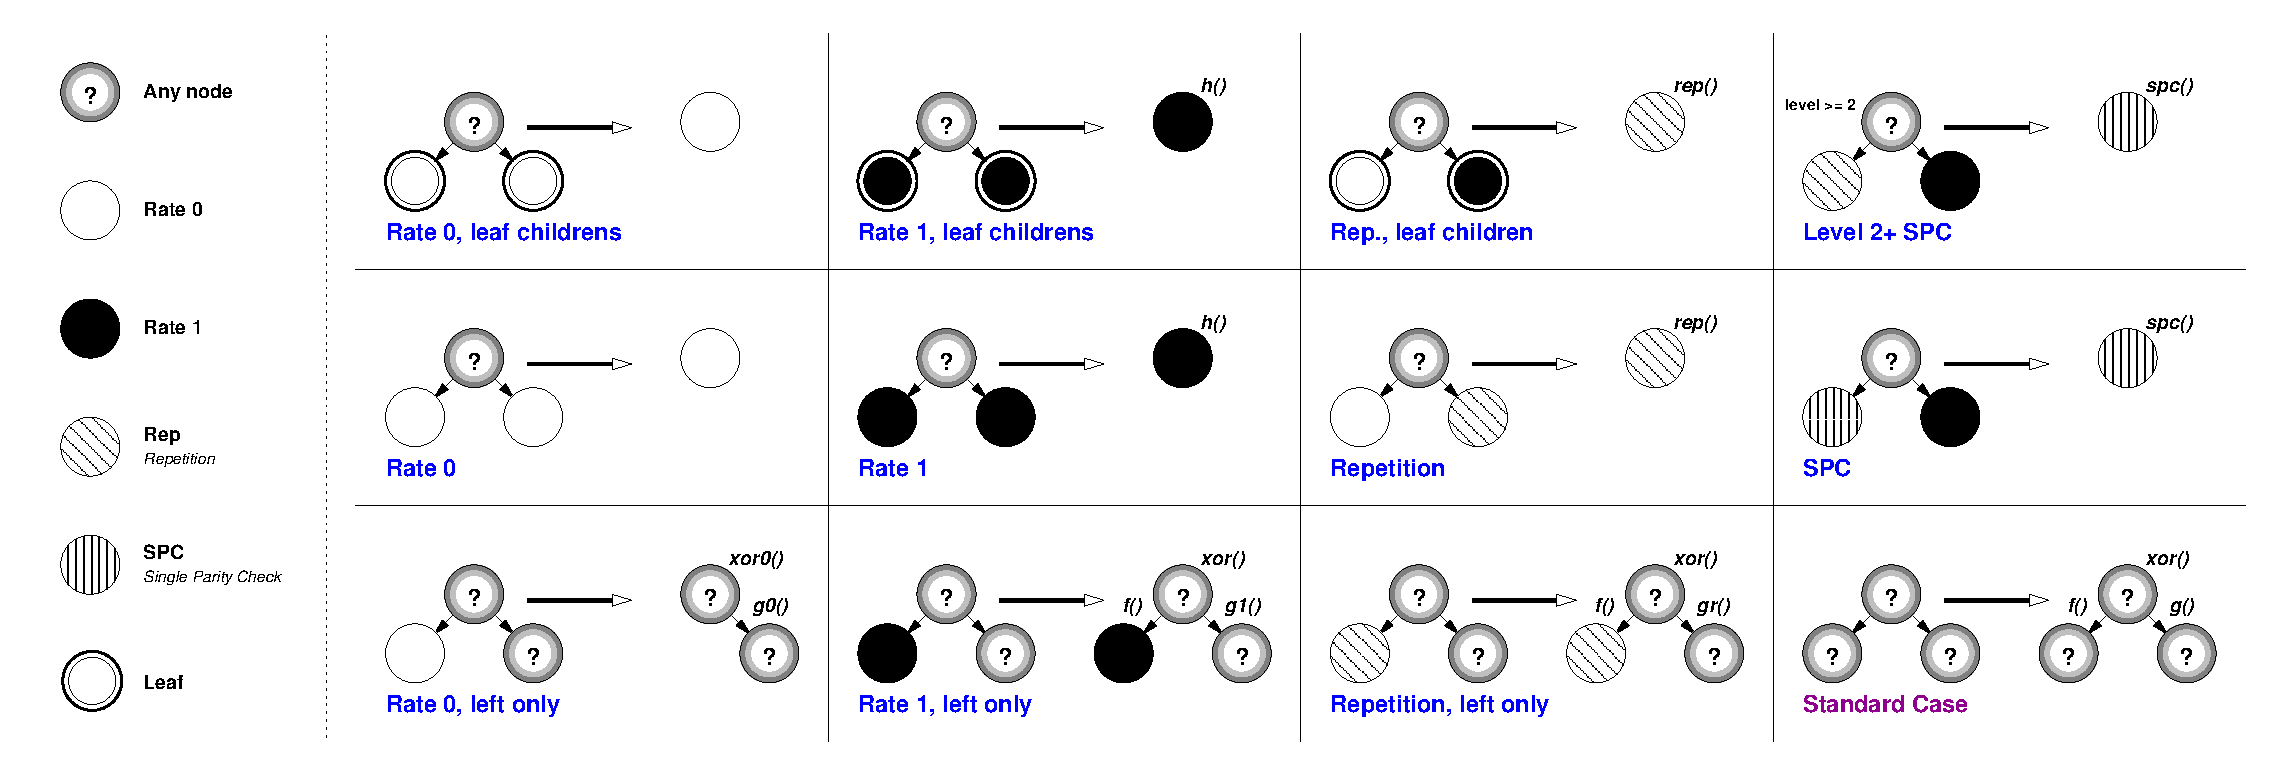
\includegraphics[width=1.0\textwidth]{polar/patterns}
  \caption{Subtree rewriting rules for processing specialization.}
  \label{fig:polar_patterns}
\end{figure}

For some sub-tree pattern configurations, the processing to be performed at the
root of such sub-trees can be simplified, or even skipped completely, for
instance when a node only has two frozen bit leaf children. To exploit such
properties, the decoder generator repeatedly applies the set of sub-tree
rewriting rules listed in Fig.~\ref{fig:polar_patterns} using a depth first
traversal to alter the node tags, until no rewriting rule applies anymore.

Each rewriting rule defines a subtree pattern \emph{selector}, a new \emph{tag}
for the subtree root, and the $f$, $g$, and $h$ \emph{processing functions} to
be applied, simplified or skipped for this node in the resulting decoder. A
\emph{null} $f$ (resp. $g$) function cuts the left (resp. right) child of the
node. From an implementation point of view, a rule is defined as a class, with a
\texttt{match} function, and a set of functions $f$, $g$, and $h$. The current
set of rewriting rules can thus easily be enriched with new rules to generate
even more specialized versions.

Patterns on the first two rows result in cutting away both children. For
instance, the first rule, named \emph{Rate~0, leaf children}, cuts the two
frozen bit leaf children of the parent node, and tag it as \emph{Rate~0} (white
node). Processing is completely skipped on this node since the values of the
bits are unconditionally known. The \emph{Repetition} rules match subtrees where
only the rightmost leaf is black (tag \emph{Rate~1}), the others being frozen
bits. In this case, the whole subtree is cut and replaced by a more simple
processing. Moreover a single, specialized $rep$ function is applied on the node
instead of the three functions $f$, $g$ and $h$. The third line describes
partial cuts and specialization. For instance, the rule ``Repetition, left
only'' specializes the $g$ and $h$ functions to use, but does not prune the
recursive children processing.

Rewriting rules are ordered by priority (left to right, then top row to bottom
row in Fig.~\ref{fig:polar_patterns}), thus if more than one rule match an
encountered subtree, the highest priority rule is applied. The priority order is
chosen such as to favor strongest computation reducing rules over rules with
minor impact, and to ensure confluence by selecting the most specific pattern
first. Rules selectors can match on node tags and/or node levels (leaf, specific
level, above or below some level). A given rule is applied at most once on a
given node.

\begin{figure}
  \centering
  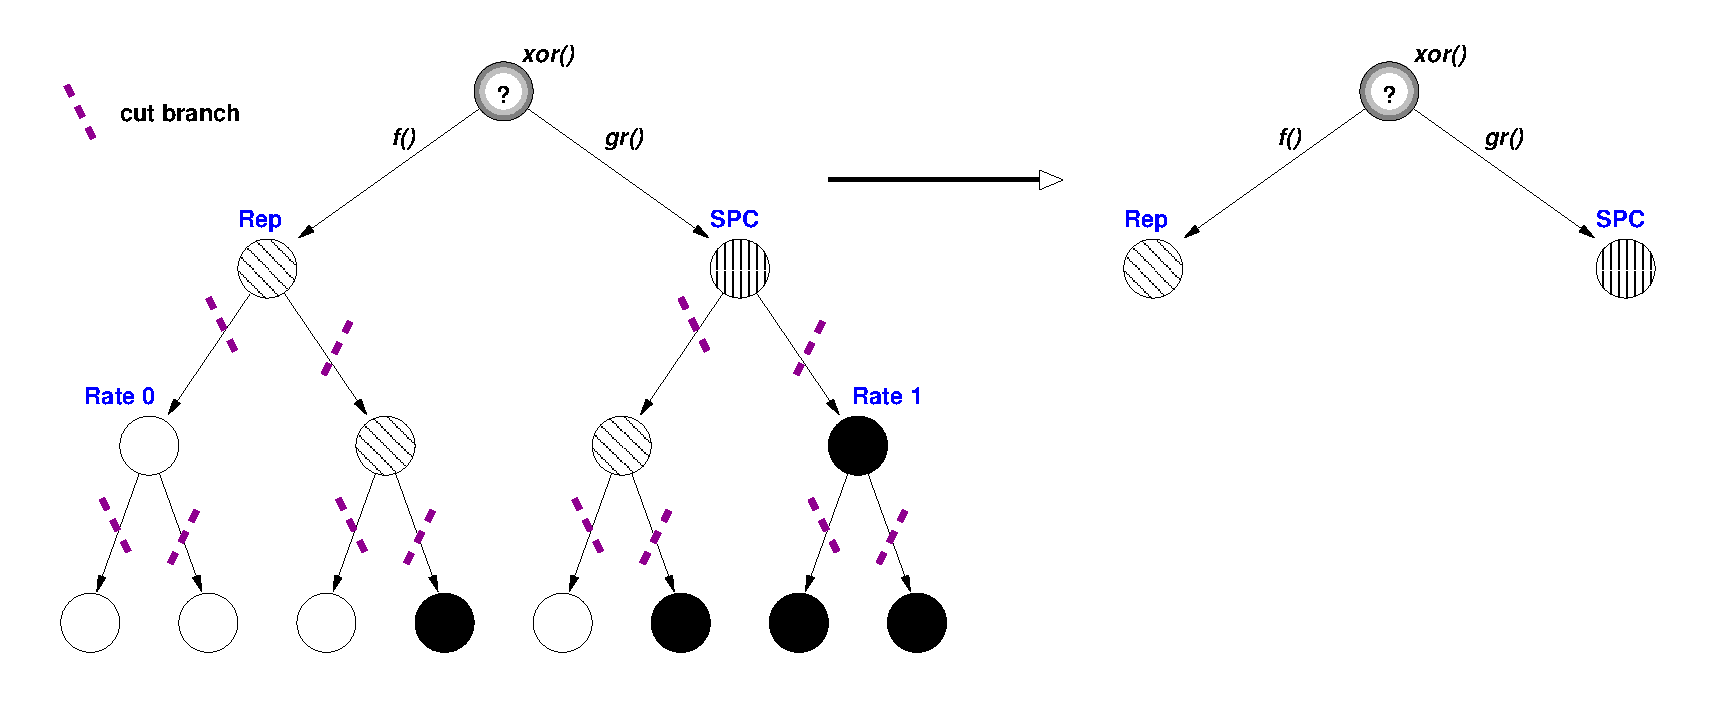
\includegraphics[width=0.70\textwidth]{polar/patterns_example}
  \caption{Generation process on a small binary tree ($N = 8$). The tree is cut
    and the computations are versioned according to the location of the frozen
    bit}
  \label{fig:polar_patterns_example}
\end{figure}

\begin{listing}
  \inputminted[frame=lines,linenos]{C++}{main/chapter2/src/polar/generated_sc_decoder.cpp}
  \caption{The final code generated corresponding to the pruned tree in
    Fig.~\ref{fig:polar_patterns_example}.}
  \label{lst:polar_patterns_example}
\end{listing}

Finally, once the tree has been fully specialized, the generator perform a
second tree traversal pass to output the resulting decoder. An example of such a
tree specialization process together with the generator output is shown in
Fig.~\ref{fig:polar_patterns_example} and in
Listing~\ref{lst:polar_patterns_example}.

\paragraph{Low Level Building blocks}
\label{sec:implem}

The main challenge in implementing P-EDGE's architecture dependent building
blocks is to provide enough flexibility to enable varied type, data layout and
optimization strategies such as intra-frame SIMDization (intra-SIMD) and
inter-frame SIMDization (inter-SIMD), without breaking the high level skeleton
abstraction. To meet this requirement, our building block library heavily relies
on generic programming and compile time specialization by the means of C++
templates, in a manner inspired by \emph{expression template}
techniques~\cite{Stroustrup2013}. Template specializations provide node
functions. Listing.~\ref{lst:polar_patterns_example} gives a example of a
generated decoder for $N = 8$, calling template instances of the node functions.
\texttt{B}:~partial sum type; \texttt{R}: LLR/$\lambda$ type;
\texttt{F}/\texttt{G}/\texttt{H}/\texttt{X}: Scalar standard SC function
versions; \texttt{FI}/\texttt{GI}/\texttt{HI}/\texttt{XI} SIMD versions.
Remaining template parameters are offsets and chunk sizes to control data
layout.

A single SIMD set is needed because \emph{SIMD routines are common to both
intra-SIMD and inter-SIMD}. In the later case, the generated decoder packs as
many frames together from the frame stream as the vector size in a transparent
manner. In both cases, offsets are fully precomputed at compile time.
\textbf{Intra-SIMD} exploits SIMD units without increasing the decoder latency,
since it still processes frames one at a time and thus preserves fine grain
frame pipelining. However, at leaf nodes and nearby, too few elements remain to
fill SIMD units. For instance, 4-way SIMD registers are fully filled only at
level 2 and above. Thus, Intra-SIMD will only be effective on trees that can be
heavily pruned from these numerous scalar nodes. \textbf{Inter-SIMD} does not
suffer from this problem, since SIMD register lanes are filled by LLRs and bits
from multiple frames instead. However, the decoder needs to wait for enough
frames to arrive, which increases latency, and to interleave the LLRs from these
frames (\emph{gather}) before proceeding. It also needs to de-interleave the
resulting data (the bits) after decoding (\emph{scatter}). Refer
to~\cite{LeGal2015a} for more details about the interleaving process.

\begin{listing}
  \inputminted[frame=lines,linenos]{C++}{main/chapter2/src/polar/f_seq.cpp}
  \caption{The C++ implementation of the $f$ function: sequential version.}
  \label{lst:polar_f_seq}
\end{listing}

\begin{listing}
  \inputminted[frame=lines,linenos]{C++}{main/chapter2/src/polar/f_simd.cpp}
  \caption{The C++ implementation of the $f$ function: SIMD version.}
  \label{lst:polar_f_simd}
\end{listing}

The framework instantiates scalar or SIMD functions as appropriate (hence the
two sets of functions). These two sets of functions are themselves
\emph{independent on the element type}. Scalar functions are
datatype-parametered templates. SIMD functions use the template-based MIPP
intrinsics wrapper library developed by one of the authors to benefit from SSE,
AVX, AVX-512 and NEON flavors SIMD instruction sets in a portable and extensible
manner. As an example, the generic scalar and SIMD implementations of the $f$
function are shown in Listing.~\ref{lst:polar_f_seq} and
Listing.~\ref{lst:polar_f_simd}. We also tried an auto-vectorized approach but even
if all the routines were well vectorized (from the compiler report), the
performance was, at least, 3 times slower than the MIPP handwritten versions.

The decoder stores its state using two data buffers, one for the LLR values
($\lambda$) and the other for the bits (partial sums $s$). The ``logical'' tree
layout is implemented as a simple and efficient \emph{heap} vector data layout.
Traversing the tree therefore corresponds to moving through the array, at
different offsets and considering different index intervals. The LLR offset is
computed from the graph depth~$d$ (or the node vertical indexing) as follows:
%\begin{equation}
%  off_{\lambda}(d) = \begin{cases}
%    0                                         &\text{$d = 0$},\\
%    \sum\limits_{i = 1}^{d} \frac{N}{2^{i-1}} &\text{otherwise.}
%\end{cases}
%\end{equation}
\begin{equation}
  off_{\lambda}(d = 0) = 0,~off_{\lambda}(d > 0) = \sum\limits_{i = 1}^{d} \frac{N}{2^{i-1}}.
\end{equation}
Given~$l$ the lane (or the node horizontal indexing), the bit offset is
determined as follows:
\begin{equation}
  off_{s}(d,l) = \frac{N}{2^d} \times l.
\end{equation}
The LLR buffer size is $2N$ and the bit buffer is $N$, for a frame of $N$ bits.
Thus, the memory footprint per frame is:
\begin{equation}
  mem_{fp} = N \times (2 \times sizeof(LLR) + sizeof(bit)).
\end{equation}
LLRs element size is 4 bytes (float) or 1 byte (fixed point numbers). The
Inter-SIMD version also employs a \emph{bit packing} memory footprint reduction
technique~\cite{LeGal2015a} to pack several bits together by using shifts and
masking instructions.

\subsubsection{Evaluations}

\begin{itemize}
  \item 32-bit, 16-bit, 8-bit
  \item consommation énergétique ARM/x86
\end{itemize}

\paragraph{SC Energy and Dynamic}

\begin{table}
  \caption{Specifications of the \odr and the \juno boards.}
  \label{tab:polar_energy_arm_specs}
  \begin{center}
  % {\footnotesize
  \begin{tabular}{c | c | c}
                                      & \textbf{ODROID-XU+E} &          \textbf{\juno} \\
    \hline
    \multirow{2}{*}{\textbf{SoC}}     &  Samsung Exynos 5410 &               ARM64 \bl \\
                                      &      (Exynos 5 Octa) &         (dev. platform) \\
    \hline
    \multirow{1}{*}{\textbf{Arch.}}   &       32-bit, ARMv7  &           64-bit, ARMv8 \\
    \hline
    \multirow{1}{*}{\textbf{Process}} &                 28nm &  unspecified (32/28 nm) \\

    \hline
    \multirow{4}{*}{\textbf{\big}}    &  4xCortex-A15 MPCore &     2xCortex-A57 MPCore \\
                                      &   freq. [0.8-1.6GHz] &     freq. [0.45-1.1GHz] \\
                                      &   L1I 32KB, L1D 32KB &      L1I 48KB, L1D 32KB \\
                                      &               L2 2MB &                  L2 2MB \\
    \hline
    \multirow{4}{*}{\textbf{\little}} &   4xCortex-A7 MPCore &     4xCortex-A53 MPCore \\
                                      &   freq. [250-600MHz] &      freq. [450-850MHz] \\
                                      &   L1I 32KB, L1D 32KB &      L1I 32KB, L1D 32KB \\
                                      &             L2 512KB &                  L2 1MB \\
  \end{tabular}
  % }
  \end{center}
\end{table}

\begin{table}
  \caption{Characteristics for each cluster ($T_i$ is the information
    throughput), for dyn. decoder. $N = 4096$, rate $R = 1/2$. The RAM
    consumption is not included in $E_b$ and in $P$.}
  \label{tab:polar_energy_results}
  \begin{center}
  %{\footnotesize
  \begin{tabular}{c | c | c | c | c | c}
    \textbf{Cluster} &
    \textbf{Impl.} &
    $\boldsymbol{T_i}$ \textbf{(Mb/s)} &
    $\boldsymbol{l}$   \textbf{($\boldsymbol{\mu}$s)} &
    $\boldsymbol{E_b}$ \textbf{(nJ)} &
    $\boldsymbol{P}$   \textbf{(W)}\\
    \hline
    \multirow{3}{*}{\textbf{A7-450MHz}}  & seq.  &  3.1 &  655 &  37.8 & 0.117 \\
                                         & intra & 13.0 &  158 &   9.5 & 0.123 \\
                                         & inter & 21.8 & 1506 &   6.0 & 0.131 \\
    \hline
    \multirow{3}{*}{\textbf{A53-450MHz}} & seq.  &  2.1 &  966 &  29.0 & 0.062 \\
                                         & intra & 10.1 &  203 &   7.0 & 0.070 \\
                                         & inter & 17.2 & 1902 &   5.1 & 0.088 \\
    \hline
    \multirow{3}{*}{\textbf{A15-1.1GHz}} & seq.  &  7.5 &  274 & 122.0 & 0.913 \\
                                         & intra & 35.2 &   58 &  28.2 & 0.991 \\
                                         & inter & 62.8 &  522 &  17.4 & 1.093 \\
    \hline
    \multirow{3}{*}{\textbf{A57-1.1GHz}} & seq.  &  9.2 &  222 &  78.9 & 0.730 \\
                                         & intra & 39.2 &   52 &  21.1 & 0.826 \\
                                         & inter & 65.1 &  503 &  14.2 & 0.923 \\
    \hline
    \multirow{3}{*}{\textbf{i7-3.3GHz}} & seq.  &  36.3 & 56.5 & 235.4 &  8.532 \\
                                        & intra & 221.8 &  9.2 &  40.5 &  9.017 \\
                                        & inter & 632.2 & 51.8 &  15.8 &  9.997 \\
  \end{tabular}
  %}
  \end{center}
\end{table}

Table~\ref{tab:polar_energy_results} gives an overview of the decoder behavior
on different clusters and for various implementations. The code is always single
threaded and only the 8-bit fixed-point decoders are considered, since 32-bit
floating-point versions  are 4 times more energy consuming, on average. The
sequential version is mentioned for reference only, as the  throughput $T_i$ is
much higher on vectorized versions. Generally the inter-frame SIMD strategy
delivers better performance at the cost of a higher latency $l$.
Table~\ref{tab:polar_energy_results} also compares the energy consumption of
\little and \big clusters. The A53 consumes less energy than the A7 and the A57
consumes less energy than the A15, respectively. This can be explained by
architectural improvements brought by the more recent ARM64 platform. Despite
the fact that the ARM64 is a development board, the ARM64 outperforms the ARM32
architecture. Finally we observe that the power consumption is higher for the
inter-frame version than for the intra-frame one because it fills the SIMD units
more intensively, and the SIMD units consume more than the scalar pipeline.

For comparison, the results for the Intel Core i7-4850HQ, using SSE4.1
instructions (same vector length as ARM NEON vectors) are also included. Even if
the i7 is competitive with the ARM big cores in term of \textit{energy-per-bit}
($E b$), these results show it is not well suited for the low power SDR systems
because of its high power requirements.

\begin{table}
  \caption{Comparison of 8-bit fixed-point decoders with intra-frame
    vectorization. $N = 32768$ and $R = 5/6$.}
  \label{tab:polar_energy_comparison}
  \begin{center}
  %{\footnotesize
  \begin{tabular}{c | c | c | c | c | c}
    \textbf{Decoder} &
    \textbf{Platform} &
    \textbf{Freq.} &
    \textbf{SIMD} &
    $\boldsymbol{T_i}$ \textbf{(Mb/s)} &
    $\boldsymbol{l}$   \textbf{($\boldsymbol{\mu}$s)}\\
    \hline
    \cite{Giard2014} & i7-2600   & 3.4Ghz & SSE4.1 &         204  &  135 \\
    \hline
    this work        & i7-4850HQ & 3.3Ghz & SSE4.1 & \textbf{580} &   47 \\
    \hline
    this work        & A15       & 1.1Ghz & NEON   &          70  &  391 \\
    \hline
    this work        & A57       & 1.1Ghz & NEON   &          73  &  374 \\
  \end{tabular}
  %}
  \end{center}
\end{table}

Table~\ref{tab:polar_energy_comparison} shows a performance comparison
(throughput, latency) with the dynamic intra-frame decoder of~\cite{Giard2014}.
On a x86 CPU, our dynamic decoder is 2.8 times faster than the state-of-the-art
decoder. Even if we used a more recent CPU, we also used the same set of
instructions (SSE4.1) and the frequencies are comparable.

\begin{figure}
  \centering
  \includegraphics[width=0.70\textwidth]{polar/sc_energy_implems_vs/sc_energy_implems_vs}
  \caption{Variation of the \emph{energy-per-bit} for different frame sizes and
    impl.: intra-/inter-frame, dyn. code on/off, on A15 @ 1.1GHz. Fixed rate
    $R = 1/2$.}
  \label{plot:polar_sc_energy_implems_vs}
\end{figure}

Figure~\ref{plot:polar_sc_energy_implems_vs} shows the \emph{energy-per-bit}
consumption depending on the frame size $N$ for the fixed rate $R = 1/2$. In
general, the energy consumption increases with the frame size. For small frame
sizes ($N$ from $2^{8}$ to $2^{14}$), the inter-frame SIMD outperforms the
intra-frame SIMD. This is especially true for $N = 2^8$ which has a low ratio of
SIMD computations over scalar computations in the intra-frame version. As the
frame size increases, the ratio of SIMD vs scalar computations increases as
well. At some point around $N = 2^{16}$ the intra-frame implementation begins
to outperform the inter-frame one, because the data for the intra-frame decoder
still fits in the CPU cache, whereas the data of the inter-frame decoder does
not fit the cache anymore. In our case (8-bit fixed point numbers and 128-bit
vector registers) the inter-frame decoders require 16~times more memory than the
intra-frame decoders. Then, for the frame size $N = 2^{20}$, both intra and
inter-frame decoders now exceed the cache capacity and the RAM power consumption
becomes more significant due to the increased number of cache misses causing RAM
transactions. In general the code generation is effective on the intra-frame
strategy whereas it is negligible on the inter-frame version of the code.

Considering those previous observations, it is more energy efficient to use
inter-frame strategy for small frame sizes, whereas it is better to apply
intra-frame strategy for larger frame sizes (comparable energy consumption with
much lower latency).

\begin{figure}
  \centering
  \includegraphics[width=1.00\textwidth]{polar/sc_energy_freq/sc_energy_freq}
  \caption{Variation of the \emph{energy-per-bit} ($E_b$) depending on the cluster
    frequency (dynamic code, intra-, inter-frame).
    A7 performance is on the left and A15 on the right. $N = 4096$ and $R = 1/2$.
    Dark colors and light colors stand for CPU cluster and RAM energy consumption,
    resp.}
  \label{plot:polar_sc_energy_freq}
\end{figure}

Figure~\ref{plot:polar_sc_energy_freq} shows the impact of the frequency on the
energy, for a given value of frame size $N=4096$ and code rate $R=1/2$. On both
A7 and A15 clusters, the supply voltage increases with the frequency from 0.946V
to 1.170V. The A7 \little cluster shows that the energy consumed by the system
RAM is significant: At 250MHz it accounts for half of the energy cost. Indeed,
at low frequency, the long execution time due to the low throughput causes a
high dynamic RAM refreshing bill. It is therefore more interesting to use
frequencies higher than 250MHz. For this problem size and configuration, and
from an energy-only point of view, the best choice is to run the decoder at
350MHz. On the A15 \big cluster, the energy cost is mainly driven by the CPU
frequency, while the RAM energy bill is limited compared to the CPU.

Thus, the bottom line about energy vs frequency relationship is: On the \little
cluster it is more interesting to clock the CPU at high frequency (higher
throughput and smaller latency for a small additional energy cost); On the
\big cluster, where the RAM consumption is less significant, it is better to
clock the CPU at a low frequency.

\begin{figure}
  \centering
  \includegraphics[width=0.70\textwidth]{polar/sc_energy_rate/sc_energy_rate_N32768}
  \caption{Variation of the \emph{energy-per-bit} ($E_b$) for $N = 32768$
    depending on the rate $R = K / N$ (various impl.: intra-, inter-frame, code
    gen. on). Running on A7, A53 and A57 @ 450MHz.}
  \label{plot:polar_sc_energy_rate}
\end{figure}

In Figure~\ref{plot:polar_sc_energy_rate} the \emph{energy-per-bit} cost
decreases when the code rate increases. This is expected because there are many
more information bits in the frame when $R$ is high, making the decoder more
energy efficient. With high rates, the SC decoding tree can be pruned more
effectively, making the decoding process even more energy efficient.
Figure~\ref{plot:polar_sc_energy_rate} also compares the ARM A7, A53 and A57
clusters for the same 450MHz frequency (note: this frequency is not available on
the A15). The \little A7 is more energy efficient than the \big A57, and the
\little A53 is itself more energy efficient than the \little A7
($E_{b_{A53}} < E_{b_{A7}} < E_{b_{A57}}$).

\begin{figure}
  \centering
  \begin{tikzpicture}
  \tkzKiviatDiagram[rotate         = 90,
                    scale          = 0.70,
                    label distance = 0.5cm,
                    label space    = 5.7cm,
                    font           = \footnotesize,
                    radial         = 5,
                    gap            = 1,
                    lattice        = 4]{Larger SNR range,
                                        Lower memory footprint,
                                        Lower latency,
                                        Lower energy per bit,
                                        Higher throughput}
  \tkzKiviatLine[ultra thick,color=red,mark=none,fill=red!20,opacity=.3](4,2,1,3,3)
  \tkzKiviatLine[ultra thick,color=blue,fill=blue!20,opacity=.3](4,4,3,1,1)
  \tkzKiviatLine[dotted,ultra thick,color=blue](2,3,4,2,2)
  \tkzKiviatLine[dotted,ultra thick,color=red](2,1,2,4,4)
  \end{tikzpicture}
  \caption{\label{fig:polar_sc_colgate}Ranking of the different approaches along
    5 metrics. In red, inter-frame vectorization performance and in blue,
    intra-frame performance. Solid color is for the dynamic versions, dotted is
    for the generated versions. Each version is sorted along each of the 5 axes
    and the best version for one axe is placed further from the center.}
\end{figure}

Figure~\ref{fig:polar_sc_colgate} presents a qualitative summary of the
characteristics of the different code versions, for intra-/inter-frame
vectorization, generated or dynamic code. For instance, if the size of
the memory footprint is an essential criterion, the dynamic intra-frame
code exhibits the best performance.

To sum up, the dynamic implementations provides efficient trade-off between
throughput, latency and energy depending on code length. It was demonstrated by
previous benchmarks. Both implementations provide low-energy and low-power
characteristics compared to previous works in the field on x86 processors
\cite{Sarkis2014,Giard2014,Sarkis2014a,LeGal2014,LeGal2015a,Cassagne2015c}.
Whereas the throughput on a single processor core is reduced compared to x86
implementations, ARM implementations must fulfil a large set of SDR applications
with limited throughputs and where the power consumption matters. Finally, it is
important to notice that multi-core implementations of the proposed ARM decoders
is still possible on these ARM targets to improve the decoding throughputs.

\paragraph{SC inter/intra-SIMD Generated (aka Unrolled)}

In this section we first describe the protocol we used, after that we provide a
performance comparison between the state-of-the-art and P-EDGE. At the end we
discuss the exploring capabilities of our framework.

\begin{table}
  \begin{center}
  %{\scriptsize
  \begin{tabular}{c|c|c|c}
           & x86-based              & ARMv7-based             & prev. work arch.~\cite{Sarkis2014}\\
  \hline
  CPU      & Intel Xeon E31225      & ARM Cortex-A15          & Intel Core i7-2600                \\
           & 3.10Ghz                & MPCore~2.32GHz          & 3.40GHz                           \\
  Cache    & 32KB L1I/L1D, 256KB L2 & 32KB L1I/L1D, L2 1024KB & 32KB L1I/L1D, L2 256KB            \\
           & L3 6MB                 & No L3                   & L3 8MB                            \\
  Compiler & GNU g++~4.8            & GNU g++~4.8             & GNU g++~4.8                       \\
  \hline
  % Flags for 32-bit& \texttt{-std=c++11 -Ofast -funroll-loops -mavx}\\
  % Flags for 8-bit & \texttt{-std=c++11 -Ofast -funroll-loops -msse4.1}\\
  \end{tabular}
  %}
  \end{center}
  \caption{Performance evaluation platforms.}
  \label{tab:polar_sc_gen_thr_specs}
  % \vspace{-1.5em}
\end{table}

The platforms used for performance evaluation are shown in
Table~\ref{tab:polar_sc_gen_thr_specs}. Unless stated otherwise, each measure is
obtained as the best of ten runs of a 10~second simulation, taking into account
frame loading and result storing. SNR (Signal Noise Ratio) is set to 2.5~dB for
tests with 1/5 and 1/2 rates, and to 4.0 dB for the 5/6, 0.84, and 9/10 rate
tests. Colors differentiate the codes rates of the Polar Code, point shapes
differentiate decoder types (Intra-SIMD vs Inter-SIMD).

\subparagraph{Comparison between P-EDGE and the State of the Art}

\begin{figure}[htp]
  \includegraphics[width=1.00\textwidth]{polar/sc_gen_thr_intra/sc_gen_thr_intra}
  \caption{Performance comparison between several code rates of 32-bit floating
    point decoding stages (running on the Intel\R Xeon\R CPU E31225 and,
    respectively, on the Nvidia\R Jetson TK1\R CPU A15).}
  \label{plot:polar_sc_gen_thr_intra}
\end{figure}

\begin{table}
  \begin{center}
  \begin{tabular}{c c c c}
    \hline
    $(N, K)$                        & Decoder                      & Info T/P (Mb/s) & Latency ($\mu$s)\\
    \hline
  %%this performance is included in the graphs
  % \multirow{2}{*}{(2048, 1024)}   & prev. work~\cite{Sarkis2014} & 147             & 7               \\
  %                                 & this work                    & 195             & 5               \\
  % \hline
  %%this performance is included in the graphs
  % \multirow{2}{*}{(2048, 1707)}   & prev. work~\cite{Sarkis2014} & 335             & 5               \\
  %                                 & this work                    & 402             & 4               \\
  % \hline
    \multirow{2}{*}{(16384, 14746)} & prev. work~\cite{Sarkis2014} & 292             & 50              \\
                                    & this work                    & 341             & 43              \\
    \hline
    \multirow{2}{*}{(32768, 27568)} & prev. work~\cite{Sarkis2014} & 220             & 125             \\
                                    & this work                    & 241             & 114             \\
    \hline
    \multirow{2}{*}{(32768, 29492)} & prev. work~\cite{Sarkis2014} & 261             & 113             \\
                                    & this work                    & 293             & 101             \\
    \hline
  \end{tabular}
  \end{center}
  \caption{Comparing P-EDGE with a state-of-art software polar decoder, for
    codes of rate 0.84 and rate 0.9, using Intra-SIMD. The two cross marks show
    state-of-the art performance results reported in~\cite{Sarkis2014}, for
    comparison.}
  \label{tab:polar_sc_gen_thr_comparison}
\end{table}

\begin{figure}
  \includegraphics[width=1.00\textwidth]{polar/sc_gen_thr_inter/sc_gen_thr_inter}
  \caption{Performance comparison between several code rates of 8-bit fixed
    point decoding stages (running on the Intel\R Xeon\R CPU E31225 and,
    respectively, on the Nvidia\R Jetson TK1\R CPU A15). Circles show P-EDGE
    results. Triangles show our former ``handwritten'' implementation
    results~\cite{LeGal2015a}.}
  \label{plot:polar_sc_gen_thr_inter}
\end{figure}

Fig.~\ref{plot:polar_sc_gen_thr_intra} shows P-EDGE intra-frame throughput on
different architectures. Our generic framework performance outperforms previous
work decoder results (between 10\% and 25\% higher). This is confirmed in
Tab.~\ref{tab:polar_sc_gen_thr_comparison} which compares P-EDGE with the
state-of-the-art result samples for some specific rates reported
in~\cite{Sarkis2014}. The throughput of the inter-frame implementation is shown
in Figure~\ref{plot:polar_sc_gen_thr_inter} for different architectures. Again,
the results confirm that our generic approach overtakes handwritten code (also
between 10\% and 25\% higher on x86).

\begin{figure}
  \centering
  \begin{subfigure}{8cm}
    \centering
    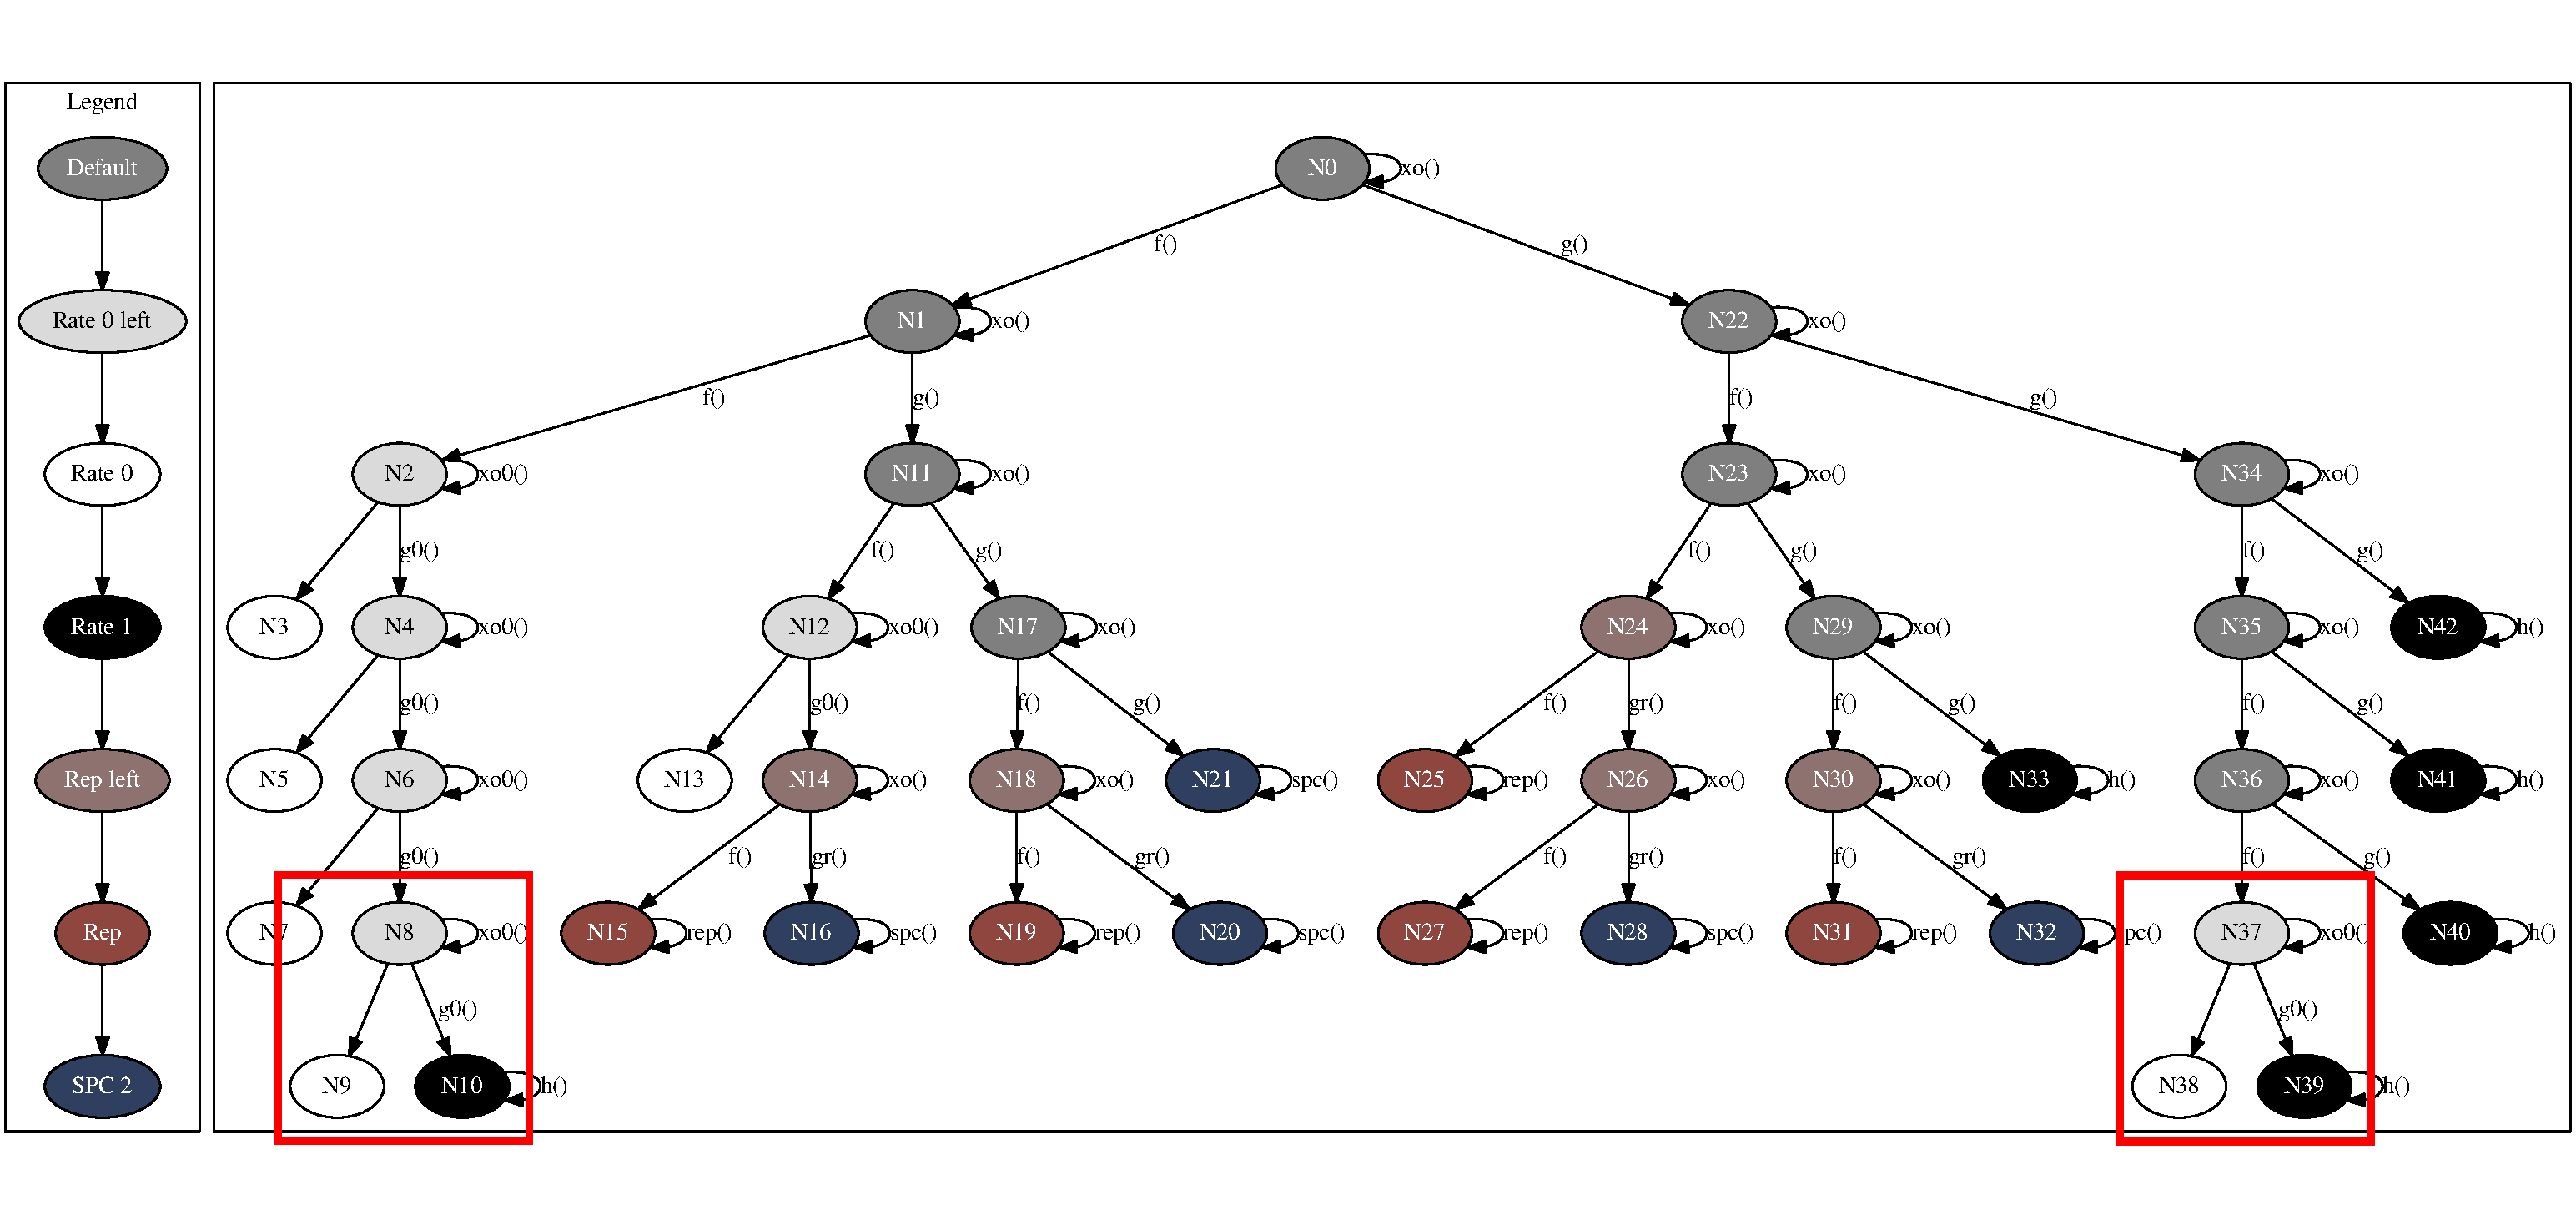
\includegraphics[width=8cm]{polar/sc_gen_compression/sc_gen_no_compression}
    \caption{Without compression.}
  \end{subfigure}
  \begin{subfigure}{4cm}
    \centering
    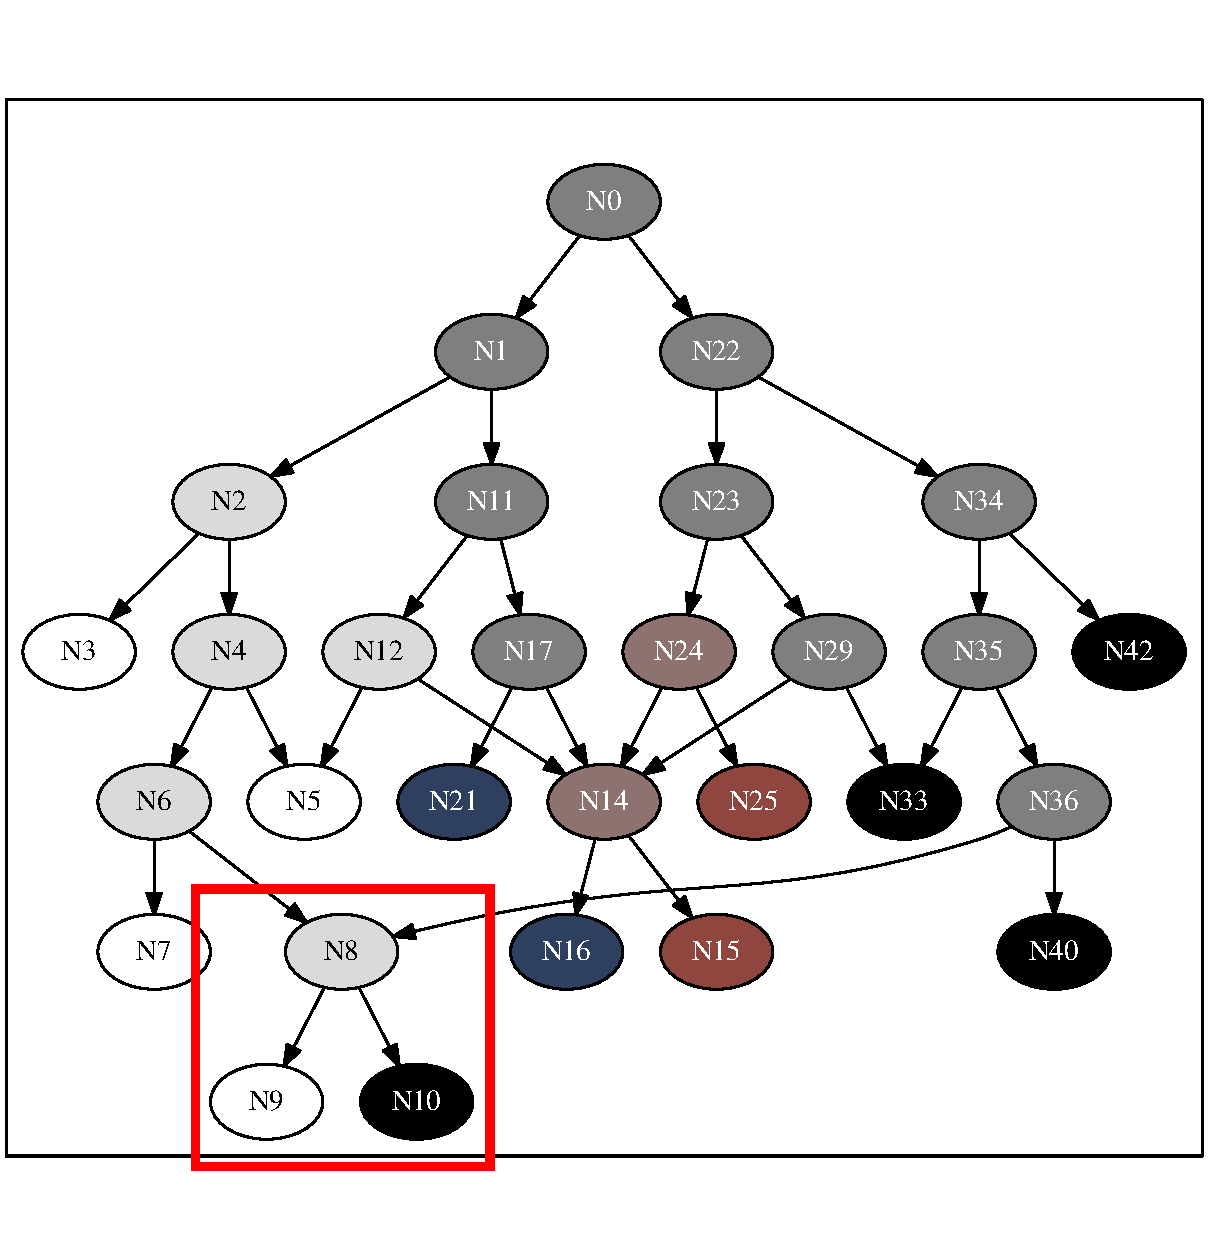
\includegraphics[width=3.725cm]{polar/sc_gen_compression/sc_gen_compression}
    \caption{With compression.}
  \end{subfigure}
  \caption{Full decoding tree representation (N = 128, K = 64) without and with
           the compression sub-tree folding algorithm.}
  \label{fig:polar_sc_gen_compression}
\end{figure}

For all the test series, the bandwidth first increases with codeword size, as
the tree pruning becomes increasingly more effective with larger trees. The
effect is stronger for Intra-SIMD where pruning also results in removing
inefficient scalar nodes. However, beyond a codeword size point which depends on
the architecture and on the selected SIMD version, performance decreases again
due to L1 cache misses, not only L1D but L1I as well. Indeed, decoders are
generated as straight-line code (no recursive calls), with all node computations
put in sequence. This improves performance for small to medium codeword size, up
to the point where the compiled binary exceeds the L1I cache size. We mitigated
this issue by reducing decoder binary sizes using two compression techniques: 1)
in the generated code, we moved the buffer offsets from template arguments to
function arguments, which enabled the compiler to factorize more function calls
than before (improvement by a factor of 10), 2) we implemented a sub-tree
folding algorithm in the generator (see
Fig.~\ref{fig:polar_sc_gen_compression}), to detect multiple occurrences of a
same sub-tree and to put the corresponding code into a dedicated function
(improvement by a factor of 5 for $N=2^{16}$, the compression ratio increases
with the size of the tree).

\begin{table}
  \begin{center}
  \begin{tabular}{ c | c | c | c | c | c | c}
    Decoder                  & $N = 2^6$ & $N = 2^8$   & $N = 2^{10}$     & $N = 2^{12}$     & $N = 2^{14}$      & $N = 2^{16}$                \\
    \hline
    inter 32-bit, $R = 1/2$  & 1 (7)     & 2 (24)      & 7 (\textbf{77})  & 9 (\textbf{254}) & 19 (\textbf{736}) & \textbf{40} (\textbf{2528}) \\
    \hline
    inter 32-bit, $R = 5/6$  & 1 (4)     & 2 (19)      & 4 (\textbf{53})  & 7 (\textbf{167}) & 16 (\textbf{591}) & 32          (\textbf{1758}) \\
    \hline
    intra 32-bit, $R = 1/2$  & 1 (4)     & 3 (16)      & 9 (\textbf{56})  & 8 (\textbf{182}) & 19 (\textbf{563}) & \textbf{38} (\textbf{1947}) \\
    \hline
    intra 32-bit, $R = 5/6$  & 1 (3)     & 3 (13)      & 6 (\textbf{38})  & 7 (\textbf{126}) & 20 (\textbf{392}) & 27          (\textbf{1365}) \\
    \hline
    inter ~8-bit, $R = 1/2$  & 1 (5)     & 2 (22)      & 7 (\textbf{72})  & 8 (\textbf{252}) & 17 (\textbf{665}) & \textbf{36} (\textbf{2220}) \\
    \hline
    inter ~8-bit, $R = 5/6$  & 1 (4)     & 2 (18)      & 4 (\textbf{51})  & 6 (\textbf{191}) & 14 (\textbf{461}) & 26          (\textbf{1555}) \\
  \end{tabular}
  \end{center}
  \caption{Code size (in KB) of the generated decoders depending on the number
    of bits $N$ per frame (code respectively compiled with AVX1 instructions for
    the 32-bit decoders and with SSE4.1 instructions for the 8-bit decoders).
    For comparison, code size without compression are shown in parentheses.}
  \label{tab:polar_sc_gen_l1i_size}
\end{table}

\begin{figure}
  \includegraphics[width=1.00\textwidth]{polar/sc_gen_l1i_size/sc_gen_l1i_size}
  \caption{P-EDGE generated decoder binary sizes depending on the frame size
    (R=1/2).}
  \label{plot:polar_sc_gen_l1i_size}
\end{figure}

Table~\ref{tab:polar_sc_gen_l1i_size} and Fig.~\ref{plot:polar_sc_gen_l1i_size}
show the binary code size of the decoders depending on $N$. The results which
exceed the 32KB of the L1I cache are highlighted in bold font. Sub-tree folding
was enabled starting from $N=2^{12}$ because there is an overhead (at run-time)
when using this technique. P-EDGE decoder code sizes without compression are
shown in parentheses: we can observe a huge improvement, until $N=2^{14}$ the
code size never exceeds the L1I cache anymore.

\paragraph{SCL Experiments and Measurements}

Throughput and latency measurements are detailed in this section. The proposed
decoder implementation is compared with the previous software decoders. Despite
the additional levels of genericity and flexibility, the proposed implementation
is very competitive with its counterparts. Note that all the results presented
in the following can be reproduced with the AFF3CT tool.

During our investigations, all the throughput and latency measurements have been
obtained on a single core of an Intel i5-6600K CPU (Skylake architecture with
AVX2 SIMD) with a base clock frequency of 3.6 GHz and a maximum turbo frequency
of 3.9 GHz. The description has been compiled on Linux with the C++ GNU compiler
(version 5.4.0) and with the following options:
\texttt{-Ofast -march=native -funroll-loops}.

\subparagraph{Fully Adaptive SCL}

Being able to easily change the list size of the SCL decoders enables the use of
the FA-SSCL algorithm. With an unrolled decoder as proposed
in~\cite{Sarkis2016}, the fully adaptive decoder would imply to generate a fully
unrolled decoder for each value of the list depth. In our work, only one source
code gives the designer the possibility to run each variation of the SCL
decoders. FA-SSCL algorithm is the key to achieve the highest possible
throughput. As shown in Table~\ref{tab:polar_scl_perfs_fixed}, with an 8-bit
fixed point representation of the decoder inner values, the achieved throughput
in the case of the ($2048$,$1723$) polar code is about $425$ Mb/s on the
i5-6600K for an $E_b/N_0$ value of $4.5$ dB. It corresponds to a FER of
$5\times10^{-8}$. This throughput is almost 2 times higher than the throughput
of the PA-SSCL algorithm. The highest throughput increase from PA-SSCL to
FA-SSCL, of about $380\%$, is in the domain where the FER is between $10^{-3}$
and $10^{-5}$. It is the targeted domain for wireless communications like LTE or
5G. In these conditions, the throughput of FA-SSCL algorithm is about $227$ Mb/s
compared to $42$ Mb/s for the PA-SSCL algorithm.

In Adaptive SCL algorithms, the worst case latency is the sum of the latency of
each triggered algorithm. In the case of PA-SSCL with $L_{max}=32$, it is just
the sum of the latency of the SC algorithm, plus the latency of the SCL
algorithm with $L=32$. In the case of the FA-SSCL algorithm, it is the sum of
the decoding latency of the SC algorithm and all the decoding latencies of the
SCL algorithm for $L={2,4,8,16,32}$. This is the reason why the worst latency of
the PA-SSCL algorithm is lower while the average latency and consequently the
average throughput is better with the FA-SSCL algorithm.

\subparagraph{Comparison With State-Of-The-Art SCL Decoders.}

\begin{table}
  \centering
  \caption{Throughput and latency comparison with state-of-the-art SCL decoders.
    32-bit floating-point representation. Code (2048,1723), $L = 32$, 32-bit
    CRC.}
  \label{tab:polar_scl_perfs_comparison}
  %{\small\resizebox{\linewidth}{!}{
  \begin{tabular}{r|r|c|c c c}
    \multirow{2}{*}{\textbf{Target}} & \multirow{2}{*}{\textbf{Decoder}} & \multirow{1}{*}{\textbf{$\bm{\mathcal{L}_{worst}}$}} & \multicolumn{3}{c}{$\bm{\mathcal{T}_i}$ (Mb/s)} \\
    \cline{4-6}
    &                                & ($\mu s$)                         & \textbf{3.5 dB} & \textbf{4.0 dB} & \textbf{4.5 dB} \\
    \hline
    % \hline
    \multirow{1}{*}{i7-4790K}
    & CA-SCL~\cite{Shen2016}         &  1572                             &  1.10           &  1.10           &   1.10          \\
    \hline
    \multirow{3}{*}{i7-2600}
    & CA-SCL~\cite{Sarkis2014b}      & 23000                             &  0.07           &  0.07           &   0.07          \\
    & CA-SSCL~\cite{Sarkis2014b}     &  3300                             &  0.52           &  0.52           &   0.52          \\
    & PA-SSCL~\cite{Sarkis2014b}     & $\approx$ 3300                    &  0.9            &  4.90           &  54.0           \\
    \hline
    \multirow{3}{*}{i7-2600}
    & CA-SCL~\cite{Sarkis2016}       &  2294                             &  0.76           &  0.76           &   0.76          \\
    & CA-SSCL~\cite{Sarkis2016}      &   433                             &  4.0            &  4.0            &   4.0           \\
    & PA-SSCL~\cite{Sarkis2016}      & $\approx$ 433                     &  8.6            & 33.0            & 196.0           \\
    \hline
%   original data
%   \multirow{4}{*}{\rotatebox[origin=c]{90}{\textbf{E5-2650}}}
%   & Proposed CA-SCL                &  6554                             &  0.27           &   0.27          &   0.27          \\
%   & Proposed CA-SSCL               &  1048                             &  1.67           &   1.67          &   1.67          \\
%   & Proposed PA-SSCL               & $\approx$ 1048                    &  4.07           &  22.9           & 124.1           \\
%   & Proposed FA-SSCL               & $\approx$ 2096                    & 14.3            & 109.8           & 180.0           \\
%   \hline
%   rescaled data from E5-2650
    \multirow{4}{*}{i7-2600}
    & This CA-SCL                    &  4819                             &  0.37           &   0.37          &   0.37          \\
    & This CA-SSCL                   &   770                             &  2.3            &   2.3           &   2.3           \\
    & This PA-SSCL                   &   847                             &  5.5            &  31.1           & 168.4           \\
    & This FA-SSCL                   &  1602                             & 19.4            & 149.0           & 244.3           \\
    \hline
    \multirow{4}{*}{i5-6600K}
    & This CA-SCL                    &  3635                             &  0.48           &   0.48          &   0.48          \\
    & This CA-SSCL                   &   577                             &  3.0            &   3.0           &   3.0           \\
    & This PA-SSCL                   &   635                             &  7.6            &  42.1           & 237.6           \\
    & This FA-SSCL                   &  1201                             & 26.1            & 207.8           & 345.5           \\
  \end{tabular}
  %}}
\end{table}

The throughput and latency of the proposed decoder compared to other reported
implementations are detailed in Table~\ref{tab:polar_scl_perfs_comparison}. For
all the decoders, all the available tree pruning optimizations are applied
excluding the \texttt{SPC4+} nodes because of the performance degradation. Each
decoder is based on a 32-bit floating-point representation. The polar code
parameters are $N=2048$, $K=1723$ and the 32-bit GZip CRC is used. The list size
is $L=32$.

The latency given in Table~\ref{tab:polar_scl_perfs_comparison} is the worst
case latency and the throughput is the average information throughput. The first
version, CA-SCL, is the implementation of the CA-SCL algorithm without any tree
pruning. As mentioned before the throughput of the proposed CA-SSCL decoder
($2.3$ Mb/s) is only halved compared to the specific unrolled CA-SSCL decoder
described in~\cite{Sarkis2016} (4.0 Mb/s). The proposed CA-SSCL decoder is
approximately 4 times faster than the generic implementation
in~\cite{Sarkis2014b} ($0.52$ Mb/s) and 2 times faster than the CA-SCL
implementation in~\cite{Shen2016} ($1.1$ Mb/s) thanks to the implementation
improvements detailed in Section~\ref{sec:implem_improv}.
Furthermore, the proposed decoder exhibits a much deeper level of genericity and
flexibility than the ones proposed in~\cite{Sarkis2014,Shen2016}. Indeed, the
following features were not enabled: the customization of the tree pruning, the
8-bit and 16-bit fixed-point representations of the LLRs, the puncturing
patterns and the FA-SSCL algorithm.

When implemented on the same target (i7-2600), the proposed PA-SSCL is
competitive with the unrolled PA-SSCL in~\cite{Sarkis2016}, being only two times
slower. This can be explained by the improvements concerning the CRC that are
described in Section \ref{subsec:crc_improv}, especially the information bits
extraction in the SC decoder. Finally, as mentioned before, the throughput of
the proposed FA-SSCL significantly outperforms all the other SCL decoders (up to
345.5 Mb/s at 4.5 dB in 32-bit floating-point).

\subsection{Generic Kernels and Multi-Kernel}

\subsubsection{Related Works}

\subsubsection{Others}

\begin{itemize}
  \item factorisation automatique de kernels et génération du code source
    associé
  \item décodeurs multi-kernels génériques SC, SCL, CA-SCL et ASCL (non
    systématique et systématique)
\end{itemize}

\section{Turbo Decoders~\cite{Cassagne2016a}}

\subsection{Related Works}

HoF turbo: \url{http://aff3ct.github.io/hof_turbo.html}

\subsection{Maximum A Posteriori Algorithm}

\begin{itemize}
  \item décodeur Turbo LTE (3G/4G)
  \item treillis
\end{itemize}

\subsection{Vectorization Strategies}

\begin{itemize}
  \item inter-SIMD
  \item décodeur inter- et intra-SIMD LTE à faible latence
\end{itemize}

\subsection{Evaluations}

\begin{itemize}
  \item 32-bit, 16-bit, 8-bit
\end{itemize}

\section{LDPC Decoders}

\subsection{Related Works}

HoF LDPC: \url{http://aff3ct.github.io/hof_ldpc.html}

\subsection{BP Algorithms}

\begin{itemize}
  \item graphe biparti
\end{itemize}

LDPC codes is a family of channel codes that is well spread in current digital
communication systems. They have been chosen in many communication standards
(Wifi, WiMAX, DVB-S2, 10Gbps Ethernet, etc.). They were also selected for the
future 5G standard data transport.

\begin{figure}
  \centering
  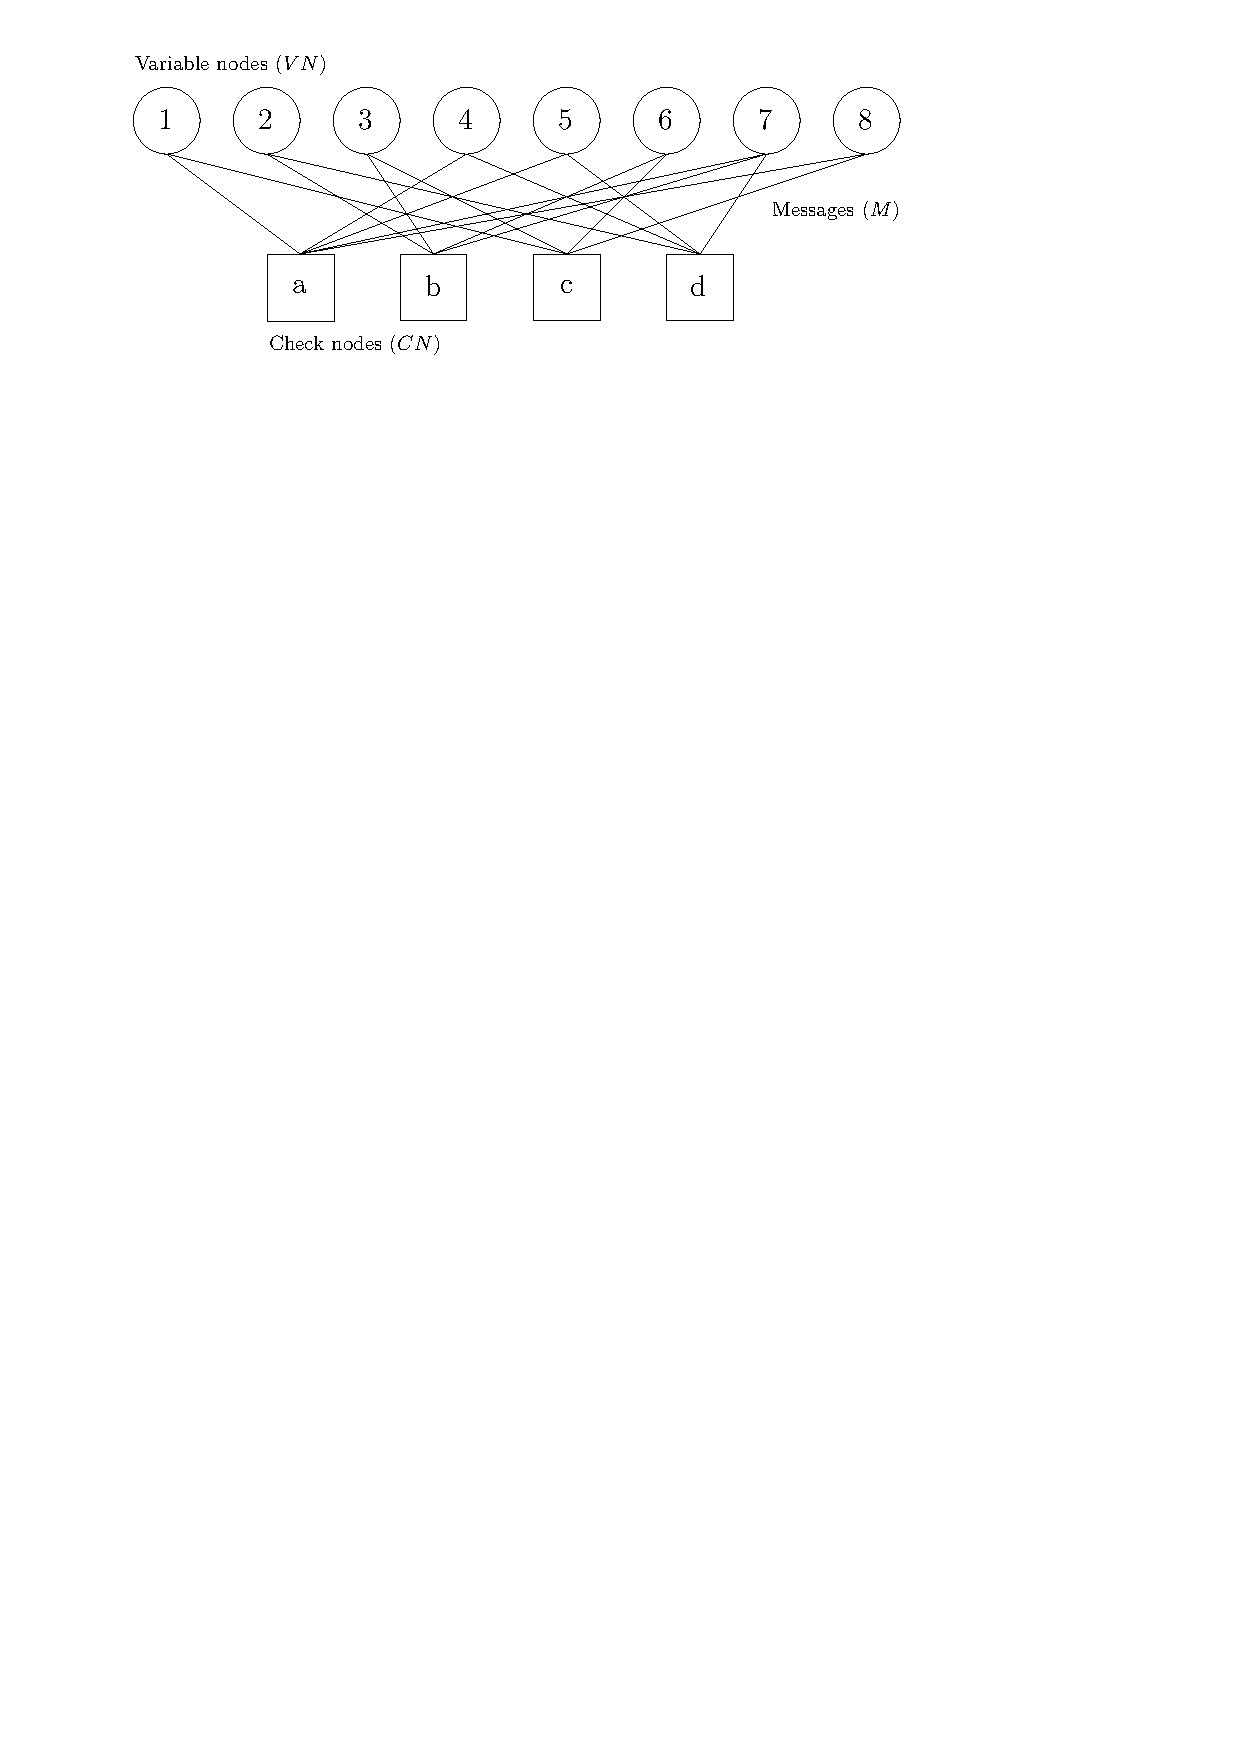
\includegraphics[width=0.60\textwidth]{ldpc/ldpc_tanner_graph}
  \caption{Tanner graph of a simple parity check $H$ matrix}
  \label{fig:LDPC}
\end{figure}

In this section the Min-Sum decoder for LDPC codes is presented. As shown in
Figure~\ref{fig:LDPC}, an LDPC code can be represented in the form of a Tanner
graph. The circles, denoted as variable nodes, represent the LLRs (the noisy
estimation of the bits in the received frames). The squares, denoted as parity
check nodes, represent the parity constraints that the variable nodes have to
verify. For instance, the check node $a$ ($CN_a$) is connected to the variable
nodes $1$, $4$, $5$, $7$ and $8$ ($VN_1, VN_4, VN_5, VN_7, VN_8$). It means that
the corresponding bits $U_1, U_4, U_5, U_7, U_8$ have to respect a parity
constraint: $U_1 \oplus U_4 \oplus U_5 \oplus U_7 \oplus U_8 = 0$. A codeword is
valid only if it respects all the parity constraints defined by the check nodes.
The LDPC code can be also represented by a \textit{parity check matrix}:
{ \begin{equation*}
H =
\begin{bmatrix}
  1&0&0&1&1&0&1&1\\
  0&1&1&0&0&1&1&0\\
  1&0&1&0&0&1&0&1\\
  0&1&0&1&1&0&1&0
\end{bmatrix}.
\end{equation*}
}
The Min-Sum decoder is an iterative message passing algorithm based on the
Tanner graph representation. Probabilistic messages ($M$) are exchanged between
the variable nodes and check nodes iteratively. Variable nodes and check nodes
apply an \textit{update rule} to compute the outgoing messages from the incoming
messages. In this section, the Min-Sum update rule is considered as well as an
horizontal layered scheduling. The original version of the Min-Sum algorithm
works on floating-point values, but it has been shown that fixed-point
simplifications have very similar decoding performance. Moreover, a fixed-point
representation enables to pack more elements into SIMD registers.

\subsection{Generic Implementation}

\begin{itemize}
  \item décodeurs génériques (BP-flooding/HL/VL) sur les "update nodes"
\end{itemize}

\subsection{Vectorization Strategies}

\begin{itemize}
  \item versions séquentielles et inter-SIMD
\end{itemize}

Listing~\ref{lst:LDPC} shows a 16-bit fixed-point LDPC decoder. This decoder
works on several frames at once. Each element of the SIMD registers corresponds
to an element of a specific frame. This approach is called the
\textit{inter-frame} vectorization. This strategy maximizes decoder throughput
at the expense of latency. Notice that the data type can be switched from
\verb|int16_t| to \verb|int8_t|, \verb|int32_t|, \verb|float| or \verb|double|.
This \MIPP feature is important for digital communication: adapting the data
type without changing the source code enables to address varying constraints
with a single source code.

\begin{listing}
  \inputminted[frame=lines,linenos]{C++}{main/chapter2/src/ldpc/bp_min_sum.cpp}
  \caption{LDPC decoder implementation with \MIPP.}
  \label{lst:LDPC}
\end{listing}

\subsection{Evaluations}

\begin{itemize}
  \item 32-bit, 16-bit
\end{itemize}

\begin{table}
  \tabcolsep=6pt
  \centering
  \caption{LDPC decoder speedups with \MIPP.}
  \label{tab:ldpc_speedups}
  %{\small
  \begin{tabular}{r|r|r|r}
                      & \textbf{\texttt{NEON}} & \textbf{\texttt{SSE}} & \textbf{\texttt{AVX}} \\ \hline
  \textbf{SIMD size}  & 8                      & 8                     & 16                    \\ \hline
  \textbf{T/P} (Mb/s) & 8.3                    & 30.3                  & 53.2                  \\ \hline
  \textbf{Speedup}    & $\times 9.7$           & $\times 8.8$          & $\times 15.2$         \\
  \end{tabular}
  %}
\end{table}

Table~\ref{tab:ldpc_speedups} presents speedups obtained with \MIPP. Ten
iterations are performed and a stop criterion was implemented for the tests
based on parity check constraints (not shown in Listing~\ref{lst:LDPC}). The $H$
matrix comes from the IEEE 802.3an standard (10Gbps Ethernet). Speedups are
close to the SIMD width. In \verb|NEON| and \verb|SSE| they even exceed it. Such
result can be explained by an optimized memory management compared to the
sequential version of the code.

\section{SCMA Demodulator~\cite{Ghaffari2019}}

\subsection{Related Works}

\subsection{Presentation}

\subsection{MPA Demodulation Algorithms}

\begin{itemize}
  \item démodulateur SCMA intra-SIMD
  \item proposition d'une approximation des calculs
\end{itemize}

\subsection{Evaluations}

\section{Discussion}
